% =====================================================================
%  DESARROLLO (versión recortada, para comparar con
%  capitulos/07-desarrollo.tex)
%
%  Recorte del 2026-10-25, para llevar el documento a 60-80 páginas:
%   - Las etapas del trabajo pasan a la entrada del capítulo, y sus tres
%     tablas (etapas, pasos en simulación y pasos con los vehículos) quedan
%     en una sola.
%   - La selección de la plataforma pasa al recorrido (DeepRacer), donde
%     ya se contaba; el cambio de la Raspberry Pi se cuenta una sola vez.
%   - El orden de puesta en marcha se une a Nav2 en el vehículo.
%   - Las cifras de odometría de los pisos 3 y 4 quedan en los resultados;
%     la espera de 1,5 s antes de verificar la llegada pasa a la
%     instrumentación.
%   - El hall del piso 2: el error es del 25 % sobre la medida real (antes
%     decía 20 %).
%   - Registro impersonal en todo el capítulo (corrección del 27 de octubre:
%     la primera persona estaba mal); la postura se dice sin «nosotros».
%   - Revisión del 27 de octubre: cambio del edificio Gregorio (pisos 2 y 3)
%     al Calatayud (pisos 3 y 4); contrato de interfaces en tabla; figuras de
%     los nodos, del planificador y de la instrumentación; cómo salen las 930
%     combinaciones y cómo se sortearon las semillas; fechas en lugar de
%     «durante meses»; menos remisiones a otras secciones y al director.
%   - Figuras y tablas con colocación [htbp] en lugar de [H], para que no
%     dejen páginas a medio llenar.
%  Ninguna figura sale del capítulo.
% =====================================================================
\chapter{Desarrollo}
\label{cap:desarrollo}

El sistema se construyó en dos semestres de 2026, con las seis fases que fijó el
anteproyecto: formulación, levantamiento de requisitos, diseño conceptual,
desarrollo progresivo, integración y pruebas, y validación con análisis de
resultados. El primer semestre, de febrero a junio, cerró las tres primeras y
empezó el desarrollo. El segundo, de agosto a octubre, hizo la integración y la evaluación con un cronograma replanificado (tabla~\ref{tab:etapas}). En esa segunda mitad, la matriz de requisitos asignó a
cada requisito la prueba que lo declara cumplido, y los criterios de la
demostración física fijaron qué debían superar los agentes físicos y hasta cuándo se tomaban datos.

\begin{table}[htbp]
  \caption{Etapas del trabajo frente a las fases del anteproyecto.}
  \label{tab:etapas}
  \footnotesize
  \begin{tabular}{@{}p{0.13\textwidth}p{0.17\textwidth}p{0.64\textwidth}@{}}
    \toprule
    \textbf{Período} & \textbf{Fase} & \textbf{Lo que se hizo} \\ \midrule
    Febrero y marzo & Planteamiento y requisitos & Anteproyecto, con el problema, la pregunta, la revisión de literatura y su sustentación; requisitos funcionales y restricciones técnicas \\ \addlinespace
    Abril & Requisitos y diseño conceptual & Análisis del DonkeyCar y de los simuladores; adopción del modelo del AWS DeepRacer y migración a ROS~2 Humble; arquitectura con servidor central y escenario de relevo \\ \addlinespace
    Mayo y junio & Desarrollo progresivo & Pasillo de la universidad en Gazebo; seguidor de paredes, descartado; sensores en el modelo del edificio Gregorio; primer mapa con SLAM \\ \addlinespace
    Agosto & Integración & En simulación: Nav2 para dirección Ackermann, contrato de interfaces, dos agentes aislados, entorno de dos pisos del edificio Gregorio, requisitos, protocolo y primera misión con relevo. Con los agentes físicos: software de la comunidad, láser y mando desde ROS~2 \\ \addlinespace
    Septiembre & Integración y validación & En simulación: campaña de treinta misiones, interfaz en un teléfono, confirmación de cambio de piso, cancelación y código congelado. Con los agentes físicos: segundo agente, banda muerta, decisión de la demostración física y primera navegación autónoma \\ \addlinespace
    Octubre & Validación & Pisos 3 y 4 del edificio Calatayud levantados con flexómetro; odometría verificada; unidad inercial; llegada verificada; media vuelta; coordinador en el portátil; campaña con los agentes físicos \\ \bottomrule
  \end{tabular}
\end{table}

\section{Recorrido del trabajo}
\label{sec:recorrido}

\subsection{La plataforma DonkeyCar y su simulador}
\label{sec:donkeycar}

El anteproyecto planteó construir los agentes sobre DonkeyCar, con una Raspberry Pi~4,
simulación en CoppeliaSim y visión con OpenCV. DonkeyCar es una plataforma
abierta de vehículos a escala con dirección tipo automóvil, orientada a la
conducción autónoma con una cámara \autocite{donkeycar}. En abril se instaló su
simulador y se condujo desde la interfaz web de la plataforma. En paralelo se empezó un modelo propio del agente para ROS~2, con el chasis, las ruedas, la
dirección y su árbol de transformaciones (figura~\ref{fig:donkeycar}).

\begin{figure}[htbp]
  \centering
  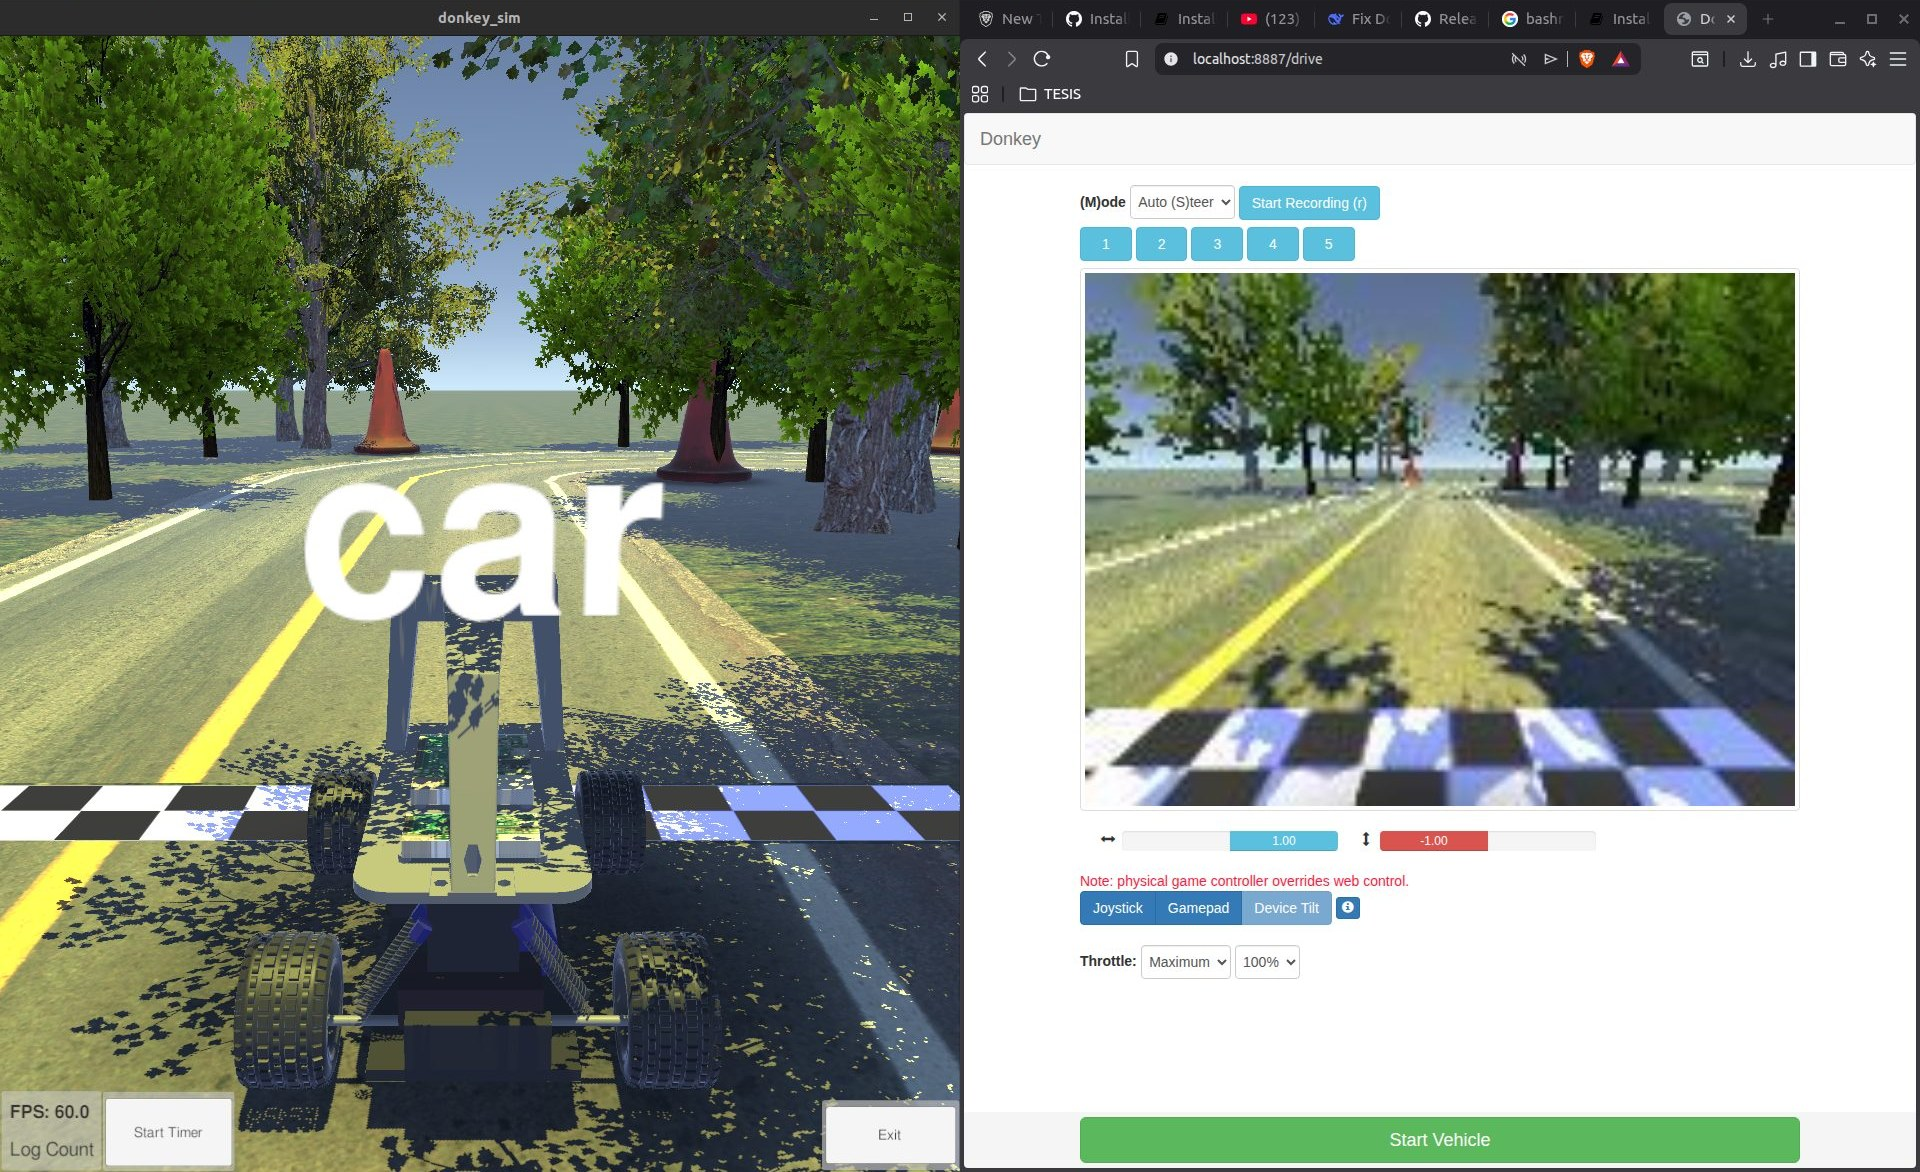
\includegraphics[height=5.2cm]{imagenes/etapa_donkeycar_simulador.jpg}\hfill
  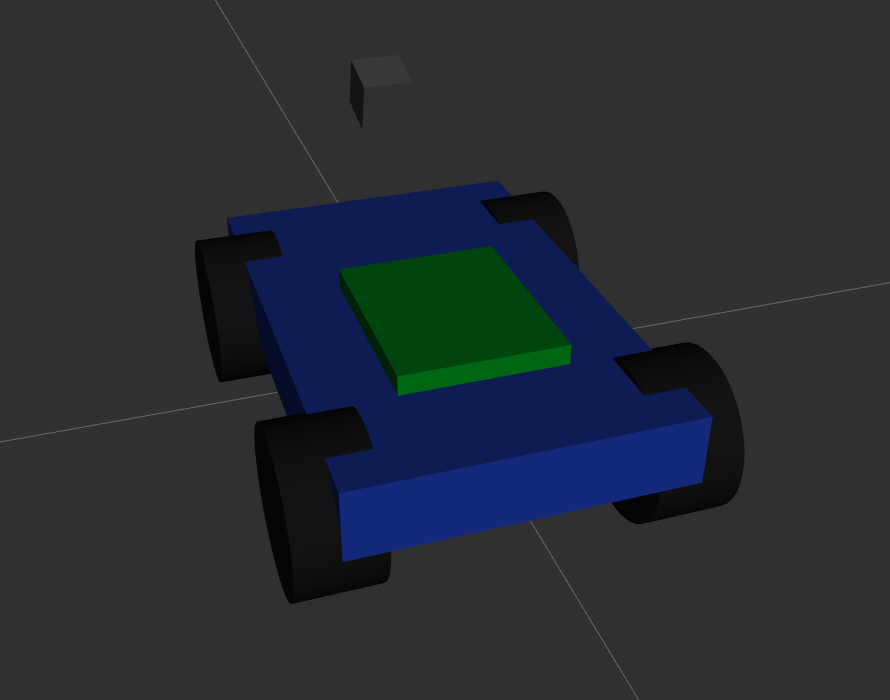
\includegraphics[height=5.2cm]{imagenes/etapa_donkeycar_modelo.png}
  \caption{Exploración de la plataforma DonkeyCar. A la izquierda, su simulador
    conducido desde la interfaz web de la plataforma, con la imagen de la cámara a bordo. A la derecha, el modelo propio del agente en el visualizador
    de ROS~2, con el chasis, las ruedas y la dirección.}
  \label{fig:donkeycar}
\end{figure}

Ese trabajo mostró tres limitaciones. El ecosistema DonkeyCar no se actualiza
desde hace años y no es compatible con las versiones recientes de ROS~2. Su
simulador no se comunica con ROS~2, así que no permite probar el mapeo, la
localización, la planificación ni la comunicación entre agentes, que son el núcleo
del proyecto. Y no existía un modelo del DonkeyCar para Gazebo con dirección
Ackermann que funcionara en ROS~2 Humble.

Para el simulador se fijaron cuatro criterios: compatibilidad con ROS~2 Humble,
vehículos con dirección Ackermann, entornos interiores y soporte para mapeo y
navegación. Entre CoppeliaSim, que proponía el anteproyecto, el simulador del
curso F1TENTH \autocite{okelly2019f1tenth} y Gazebo \autocite{koenig2004gazebo},
se eligió Gazebo por su integración directa con ROS~2 y con su sistema de control
de articulaciones. También se conservó un chasis con dirección tipo automóvil. Cada agente atiende un piso y la persona cambia de nivel por la escalera, así que ningún agente tiene que entrar a un ascensor ni subir escalones. La vuelta dentro del pasillo puede quedar a cargo de un planificador para
automóviles.

\subsection{El modelo de AWS DeepRacer y su migración a ROS~2 Humble}
\label{sec:migracion}

Una semana después se cambió al modelo del AWS DeepRacer, la decisión que hizo viable el proyecto en el tiempo disponible. Es la misma
clase de plataforma que el DonkeyCar, con chasis a escala 1:18, dirección
Ackermann, computador a bordo y software abierto. AWS publicó en código abierto su
modelo de simulación, con un complemento de cinemática Ackermann para Gazebo y
los nodos que traducen las órdenes de velocidad a los servos
\autocite{awsdeepracer2021}, y la universidad ya tenía dos. Lo que pide
el segundo objetivo, que es cinemática tipo automóvil, bajo costo y código
modificable, se cumple igual con las dos plataformas, y usar las que existían dejó
el tiempo para la coordinación. El costo fue convivir con el software del
fabricante, cuyos nodos ocupan el láser, se ejecutan con el usuario
administrador y publican sin espacio de nombres.

El software de AWS estaba escrito para ROS~2 Foxy sobre Ubuntu 20.04, y el
proyecto trabaja con Humble sobre Ubuntu 22.04. La migración necesitó tres
cambios, todos en el sistema de control de articulaciones: la orden que activa
los controladores pasó de \texttt{start} a \texttt{active}, y el componente que
publica el estado de las articulaciones cambió de nombre y de tipo. En un mundo
vacío (figura~\ref{fig:deepracer-sim}, izquierda), el modelo apareció con el láser y la cámara publicando a 62 cuadros por segundo, con un factor de tiempo
real de 1,00 y los siete controladores activos. La odometría registró 0,40~m/s
ante una orden de 0,5~m/s.

\begin{figure}[htbp]
  \centering
  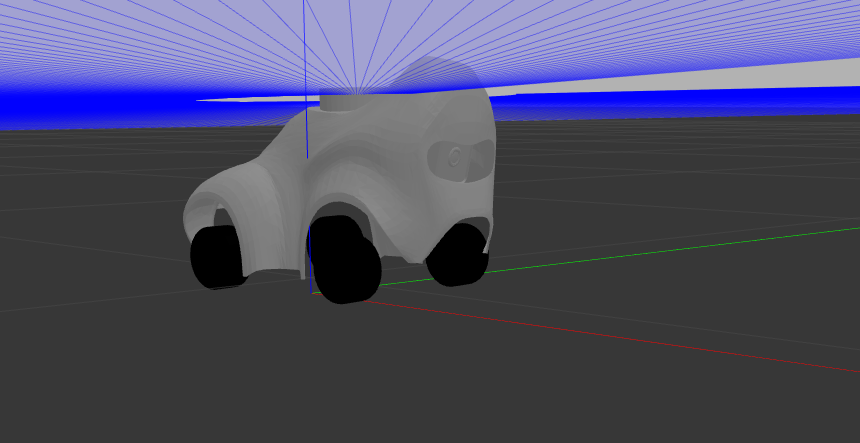
\includegraphics[height=4.6cm]{imagenes/etapa_deepracer_gazebo.png}\hfill
  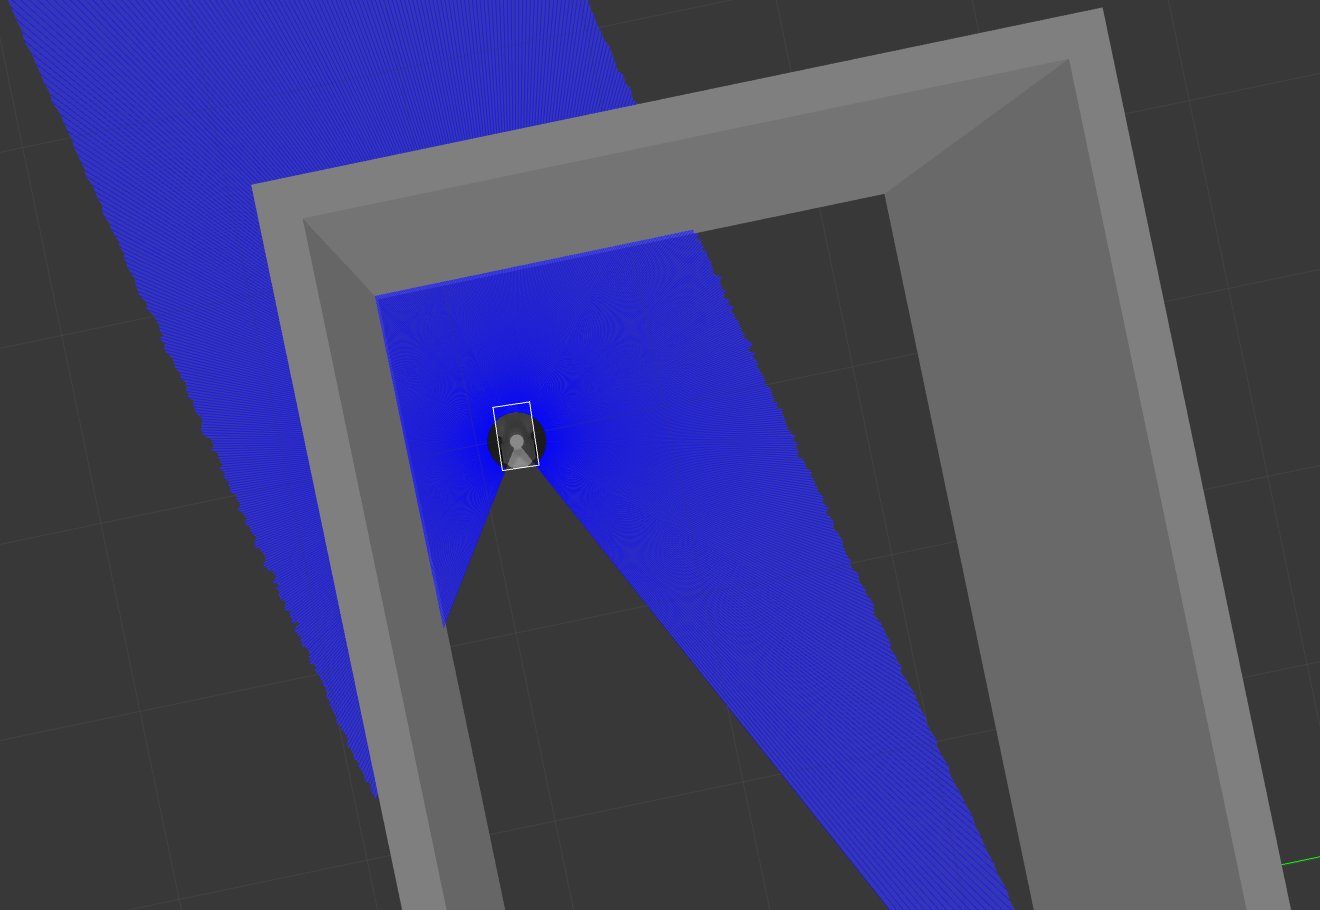
\includegraphics[height=4.6cm]{imagenes/etapa_pasillo_usta.png}
  \caption{El modelo del DeepRacer migrado a ROS~2 Humble. A la izquierda, en un
    mundo vacío, con el barrido del láser en azul. A la derecha, dentro del primer
    modelo del pasillo de la universidad, de 7 por 3~m; el sector sin barrido
    detrás del agente es el que no cubría el láser del modelo simulado.}
  \label{fig:deepracer-sim}
\end{figure}

\subsection{Los primeros entornos simulados y el seguidor de paredes}
\label{sec:primeros-entornos}

En mayo se modeló un tramo del pasillo de la universidad, de 7 por 3~m
(figura~\ref{fig:deepracer-sim}, derecha). Sobre él se programó un seguidor de paredes, como ejercicio de integración entre el láser y la cinemática del agente. La primera versión aplicaba control
proporcional-derivativo sobre un rayo lateral del láser, y saturaba el giro
porque no conocía la orientación del agente respecto a la pared. La segunda usó
la técnica de dos rayos del curso F1TENTH, que estima ese ángulo y la distancia a
la pared un metro más adelante.

En el pasillo de 7 por 3~m ninguna sintonía estabilizó al agente: el giro se
saturaba y el agente trazaba círculos o chocaba, porque su radio de giro deja
muy poco margen en 3~m de ancho. En un pasillo ampliado de 15 por 5~m convergió
por tramos, a 0,76~m de la pared frente a un objetivo de 0,5~m, y se perdía
en los extremos. La conclusión fue que un comportamiento reactivo no anticipa las restricciones de un vehículo tipo automóvil en un pasillo estrecho.
Por eso el proyecto pasó a navegar con un mapa y con un planificador que conoce
esas restricciones.

Después se modeló el primer entorno de pruebas, el piso 2 del edificio Gregorio de la universidad, donde están los salones ETM: un pasillo de 44,25~m de largo y 5,09~m de ancho. En él se comprobaron el láser, la cámara, la odometría y el árbol de transformaciones. Con ese mundo se construyó el primer mapa por localización y
mapeo simultáneos (SLAM), que se aceptó sin medirlo. Medido en septiembre,
resultó de 23,04 por 15,72~m, la mitad del largo y el triple del ancho del
pasillo. Fue la primera manifestación, sin diagnóstico entonces, de la falta de información de avance en un pasillo recto, que acabó determinando cómo se hicieron los mapas.

\subsection{La integración en simulación}
\label{sec:recorrido-sim}

El segundo semestre empezó con un cronograma replanificado, con un criterio de cierre por semana. Lo primero fue ordenar la base.
El espacio de trabajo donde se compilaba el código era una copia del repositorio
del fabricante y no un enlace al del proyecto, así que los ajustes del mapeo del
primer semestre nunca se habían ejecutado. Se enlazó al repositorio del proyecto
y se fijó el contrato de interfaces.

En agosto se aislaron los dos agentes, se construyó el entorno de dos pisos, con los pisos 2 y 3 del edificio Gregorio, y se escribieron los requisitos y el protocolo. A finales de agosto se completó la primera misión con relevo, y la campaña de treinta misiones corrió el 4 y el 5 de septiembre.

También se corrigió el modelo del agente, que tomaba la velocidad angular de la
orden estándar de ROS~2 como el ángulo del volante. Ahora el ángulo se calcula con
el modelo de bicicleta, a partir de las velocidades angular y lineal y de la
distancia entre ejes, y el error de seguimiento de las trayectorias bajó a la
mitad. La misma corrección se aplicó al nodo que mueve al agente físico.

\subsection{Del primer agente físico a la campaña con los dos}
\label{sec:recorrido-fisico}

Con los agentes físicos se trabajó en paralelo desde agosto. Se instaló el software de
la comunidad del DeepRacer \autocite{deepracercustomcar} en una Raspberry Pi~4 y
en la tarjeta original, y los agentes quedaron con su tarjeta original, con
Ubuntu 24.04 y ROS~2 Jazzy. Como la integración de
Gazebo~11 con ROS~2 no está publicada para Jazzy, desde entonces el proyecto
trabaja con dos distribuciones.

Las pruebas con los agentes físicos empezaron en los pasillos del edificio Gregorio, los mismos que se habían modelado para la simulación. Llevar allí los agentes resultó difícil por el tránsito de personas durante las pruebas, y en esos pasillos uniformes la odometría del láser no registraba el avance. Además, el modelo del piso 3 de Gregorio no correspondía a la planta real. El 2 de octubre el trabajo pasó a los pisos 3 y 4 del edificio Calatayud, que el equipo levantó con flexómetro ese mismo día. De esas medidas salieron los mapas, los mundos simulados y el catálogo de destinos de la campaña física.

En el camino hubo otros dos tropiezos: una supuesta avería que resultó ser un problema de permisos, y la saturación de la tarjeta con dos cadenas de navegación. El 21 de septiembre se decidió intentar la demostración física con seis pruebas de verificación, y la campaña con los agentes físicos corrió el 16 de octubre.

% =====================================================================
\section{Arquitectura funcional del sistema}
\label{sec:oe1}

La figura~\ref{fig:arquitectura} muestra el sistema tal como se implementó en
simulación: la interfaz por la que entra la solicitud, el coordinador que la
reparte, los dos agentes con su pila de navegación y la escalera donde ocurre el
relevo.

\begin{figure}[htbp]
  \centering
  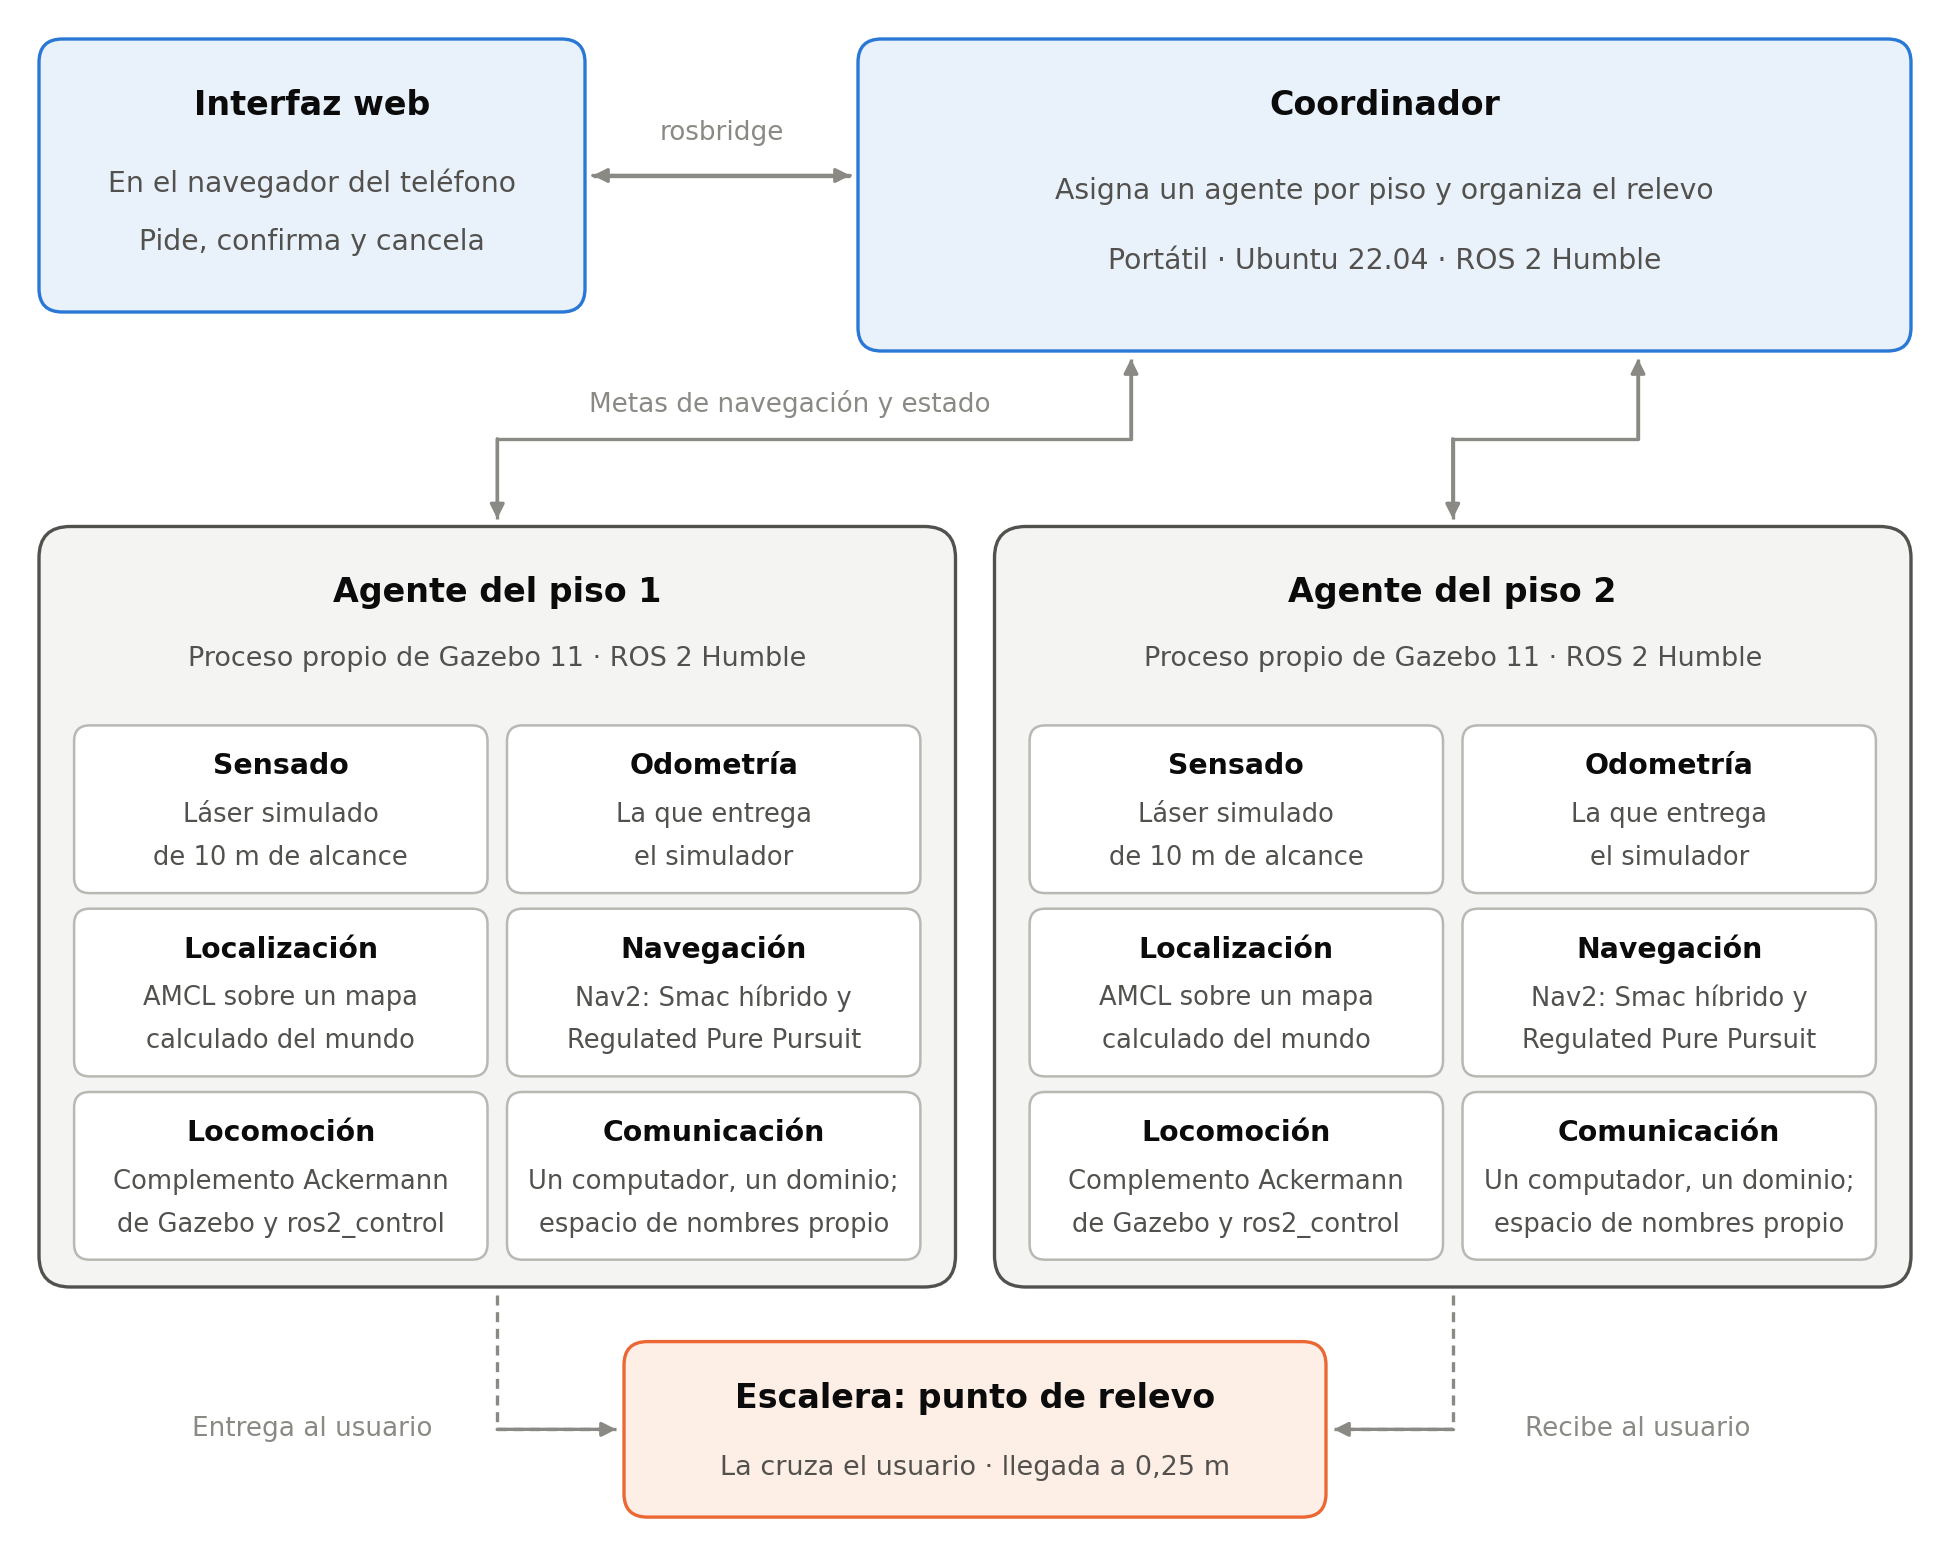
\includegraphics[width=0.86\textwidth]{imagenes/arquitectura_simulacion.png}
  \caption{Arquitectura del sistema en simulación, con un proceso de Gazebo por
    piso. Ningún agente atraviesa la zona de transición: lo que la cruza es el
    usuario, y lo que se traspasa entre agentes es la responsabilidad de guiarlo.}
  \label{fig:arquitectura}
\end{figure}

\subsection{Requisitos}

El anteproyecto no enumeró los requisitos del sistema, aunque su metodología
pedía verificar la implementación contra ellos. Se reconstruyeron al iniciar la integración a partir de los objetivos específicos, el alcance y el contrato de
interfaces. Cada requisito cita su fuente y tiene una prueba que lo declara
cumplido o no, y un requisito sin prueba no entra en la matriz.

La matriz tiene treinta y seis requisitos: veintinueve describen funciones del
sistema y siete son restricciones del alcance, como operar en interiores y en
condiciones controladas o correr la simulación en tiempo real. Al primer objetivo
le corresponden diez, sobre arquitectura, coordinación y relevo; al segundo,
seis, sobre la plataforma; al tercero, seis, sobre la interfaz; y al cuarto, siete,
sobre las métricas, el registro de cada misión y las dos campañas. La confirmación de cambio de piso y la cancelación no estaban en el anteproyecto: se añadieron al ver el sistema en uso. El avance de cada objetivo es el
promedio del estado de sus requisitos.

\subsection{El contrato de interfaces}
\label{sec:contrato}

Antes de escribir código se fijó un contrato: qué habla con qué y en qué formato.
Un coordinador central decide y manda, dos agentes, uno por nivel, ejecutan, y una
interfaz web es la vía por la que el usuario pide el servicio. La comunicación
sigue tres reglas:

\begin{enumerate}[leftmargin=*]
  \item El coordinador manda a un agente solo mediante la acción de navegación
    de ROS~2; no publica velocidades directamente. En la versión final puede
    pedirle además una media vuelta, que el agente ejecuta por su cuenta antes de navegar.
  \item La interfaz habla solo con el coordinador, nunca con los agentes.
  \item El texto que ve el usuario lo redacta el coordinador, y la interfaz lo
    muestra literal.
\end{enumerate}

La tercera regla es la que más protege el diseño: si la página interpretara el estado para decidir qué mostrar, habría dos copias de la misma lógica, y con el tiempo acabarían contradiciéndose.

El contrato se implementó como un paquete propio de mensajes de ROS~2. La acción
de guiado recibe el origen y el destino, devuelve el estado durante la misión y,
al final, el tiempo total y el número de relevos o el motivo del fallo. Cada
cambio de etapa (tabla~\ref{tab:etapas-mision}) se publica, y esas publicaciones
son las marcas de tiempo con que se calculan las métricas. La tabla~\ref{tab:contrato} reúne las interfaces entre los componentes, y la figura~\ref{fig:nodos} muestra todos los nodos del sistema en la campaña con los agentes físicos y lo que circula entre ellos.

\begin{table}[!htbp]
  \centering\footnotesize
  \caption{Interfaces del contrato entre la interfaz web, el coordinador y los agentes. \texttt{N} es el número del agente: 1 en el piso inferior y 2 en el superior.}
  \label{tab:contrato}
  \begin{tabular}{@{}p{0.36\textwidth}p{0.16\textwidth}p{0.13\textwidth}p{0.27\textwidth}@{}}
    \toprule
    \textbf{Interfaz} & \textbf{Tipo} & \textbf{Sentido} & \textbf{Contenido} \\ \midrule
    \texttt{/coordinacion/guiar\_usuario} & acción propia & interfaz $\rightarrow$ coordinador & Origen y destino; devuelve el estado durante la misión y, al final, el éxito, el tiempo total, los relevos o el motivo del fallo \\ \addlinespace
    \texttt{/coordinacion/estado\_mision} & tópico propio, 1~Hz & coordinador $\rightarrow$ interfaz & Etapa, agente activo, destino del tramo, distancia restante y texto para el usuario \\ \addlinespace
    \texttt{/coordinacion/puntos\_interes} & tópico propio, persistente & coordinador $\rightarrow$ interfaz & Catálogo de puntos de interés, con su piso \\ \addlinespace
    \texttt{/coordinacion/confirmacion\_piso} & tópico de texto & interfaz $\rightarrow$ coordinador & Confirmación de que el usuario ya cambió de piso \\ \addlinespace
    \texttt{/robotN/navigate\_to\_pose} & acción de Nav2 & coordinador $\rightarrow$ agente & Meta de cada tramo; es la única orden de movimiento \\ \addlinespace
    \texttt{/robotN/media\_vuelta} & servicio & coordinador $\rightarrow$ agente & Media vuelta antes de una meta que queda detrás \\ \addlinespace
    \texttt{/robotN/estado} & tópico propio, 2~Hz & agente $\rightarrow$ coordinador & Piso, pose en el mapa y estado del agente \\ \addlinespace
    \texttt{/robotN/odom} & odometría & agente $\rightarrow$ coordinador & Desplazamiento, con el que se marca el primer movimiento \\ \bottomrule
  \end{tabular}
\end{table}

\begin{figure}[!htbp]
  \centering
  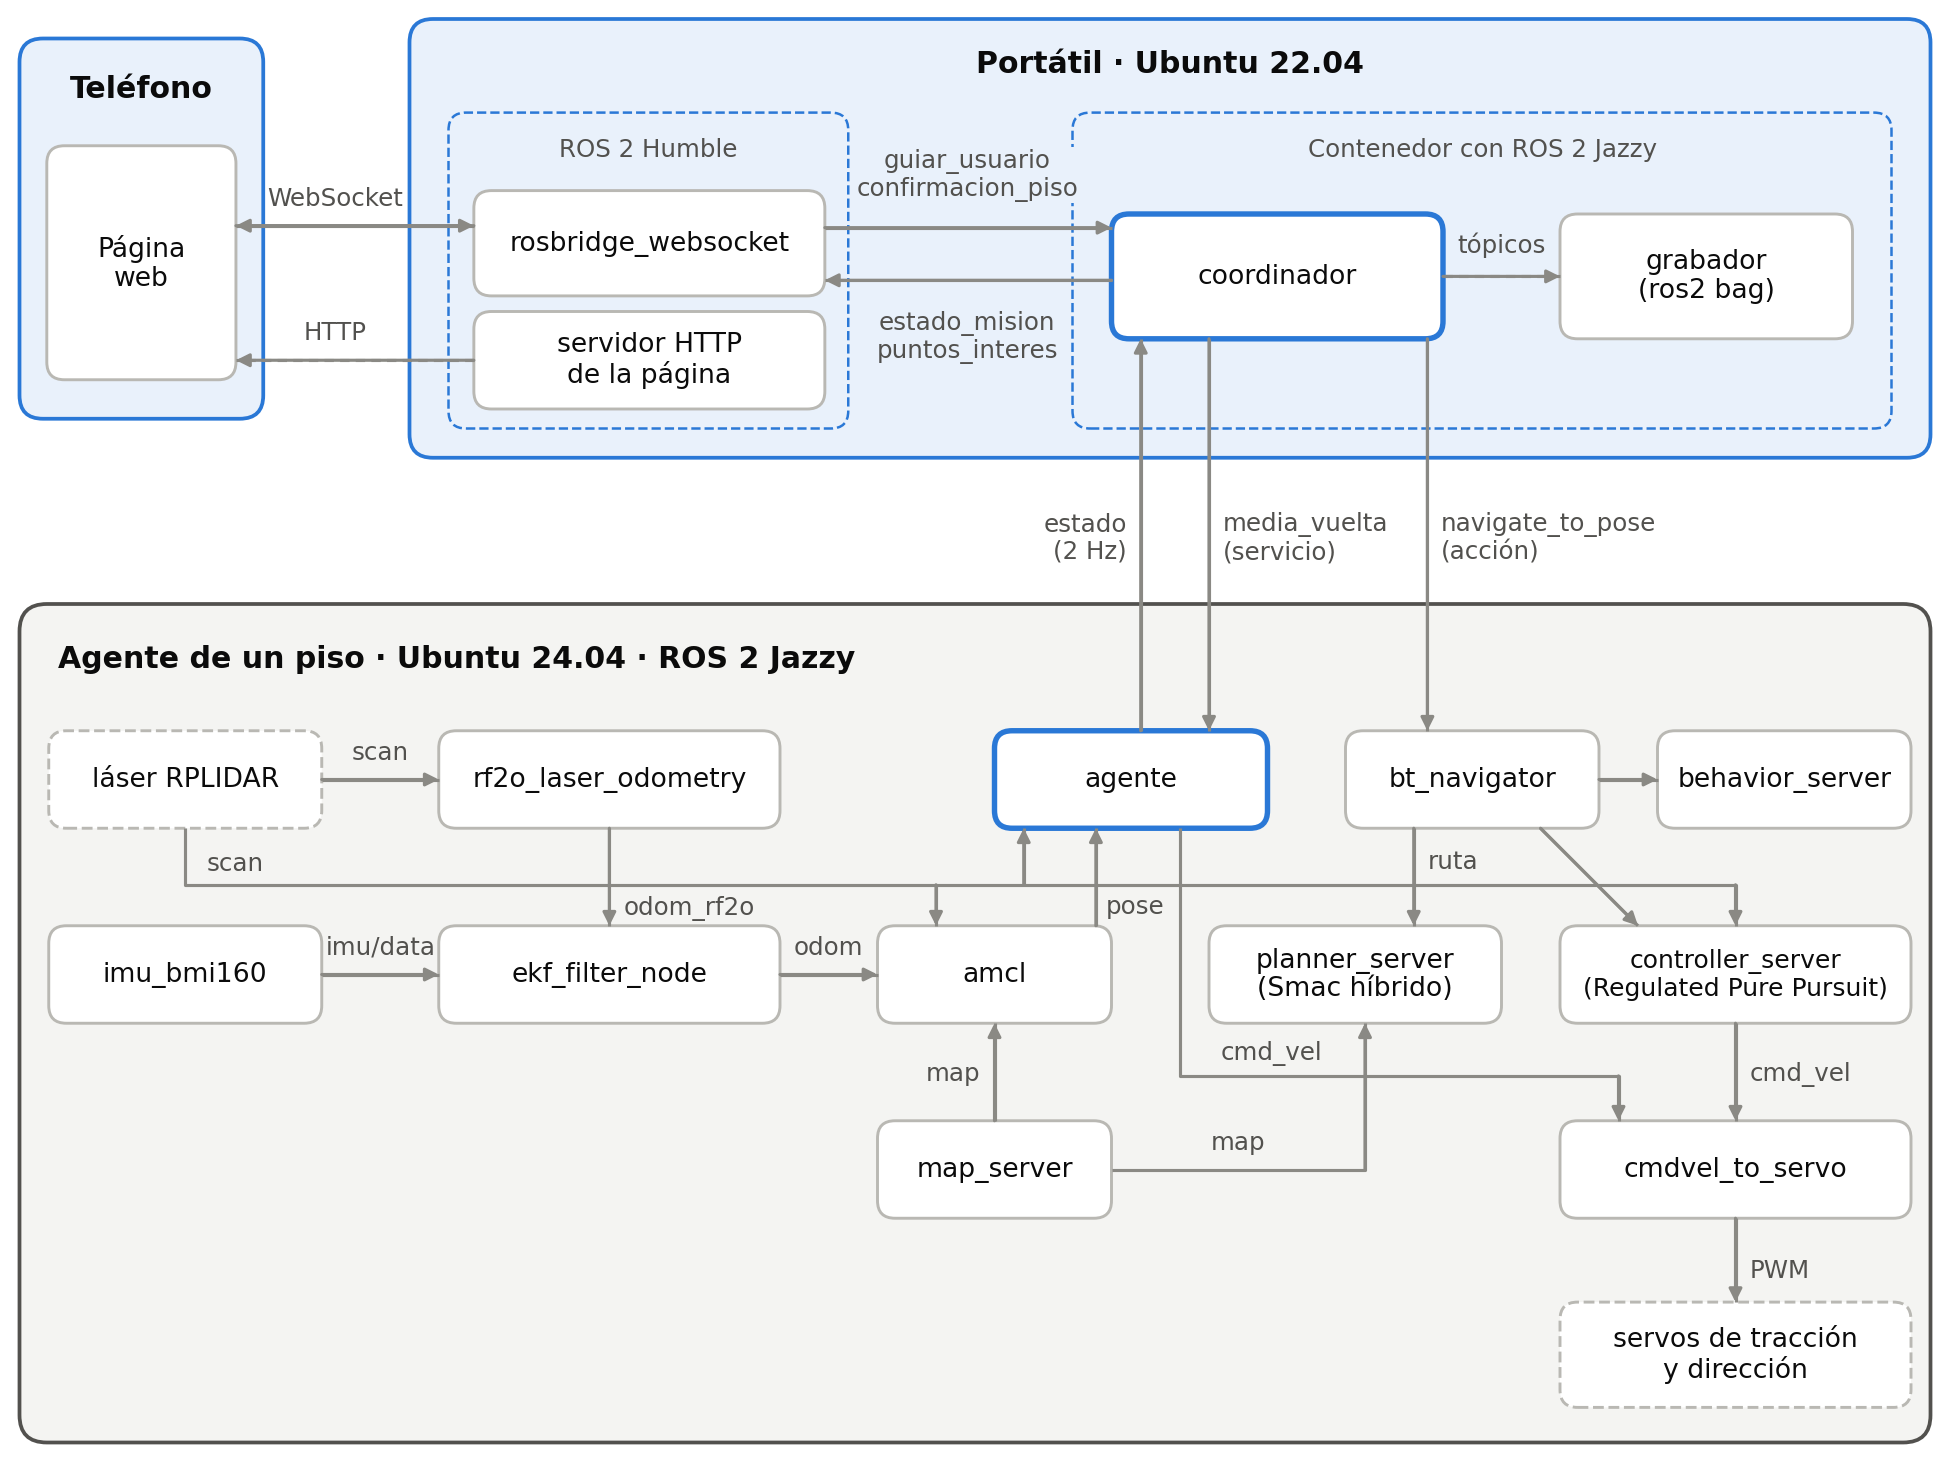
\includegraphics[width=0.96\textwidth]{imagenes/nodos_sistema.png}
  \caption{Nodos de ROS~2 del sistema en la campaña con los agentes físicos. Los dos agentes son iguales; en borde discontinuo, los componentes del fabricante. Las flechas siguen el sentido de los datos y llevan el nombre del tópico, servicio o acción. El navegador pide la ruta al planificador y su seguimiento al controlador, y la pose que estima \texttt{amcl} llega a los demás nodos por las transformadas.}
  \label{fig:nodos}
\end{figure}

\begin{table}[htbp]
  \centering\small
  \caption{Etapas de una misión, tal como las publica el coordinador.}
  \label{tab:etapas-mision}
  \begin{tabular}{@{}p{0.27\textwidth}p{0.65\textwidth}@{}}
    \toprule
    \textbf{Etapa} & \textbf{Significado} \\ \midrule
    Recibida & El coordinador aceptó la solicitud y todavía no asignó agente \\
    Primer tramo & El agente del nivel de origen va a recoger al usuario y lo guía \\
    Transferencia & El agente del otro nivel va a su punto de transferencia \\
    Esperando confirmación & El sistema espera que el usuario confirme que ya cambió de piso \\
    Segundo tramo & El agente del nivel de destino guía al usuario hasta el final \\
    Completada & La misión terminó con la llegada verificada \\
    Fallida & La misión terminó sin cumplirse, con el motivo en el texto \\
    Cancelando & El usuario canceló y el agente activo regresa a su punto de transferencia \\
    Inactiva & No hay misión en curso \\ \bottomrule
  \end{tabular}
\end{table}

\subsection{El planificador, escrito sin ROS}
\label{sec:planificador}

El relevo es el aporte declarado del proyecto, y por eso su planificación se escribió como una función pura, sin dependencia de ROS~2 ni estado propio (figura~\ref{fig:planificador}). Entran el catálogo de puntos y un par origen-destino, y salen los tramos que hay que ejecutar. Si el origen y el destino están en el mismo nivel, la misión
tiene dos tramos del mismo agente: ir a recoger al usuario y llevarlo al destino.
Si están en niveles distintos, tiene cuatro: los dos anteriores, terminando en el
punto de transferencia del nivel de origen; el desplazamiento del segundo agente
a su punto de transferencia; y el guiado final. El punto de encuentro no se negocia: es el punto de transferencia declarado de cada nivel en el catálogo.

\begin{figure}[!htbp]
  \centering
  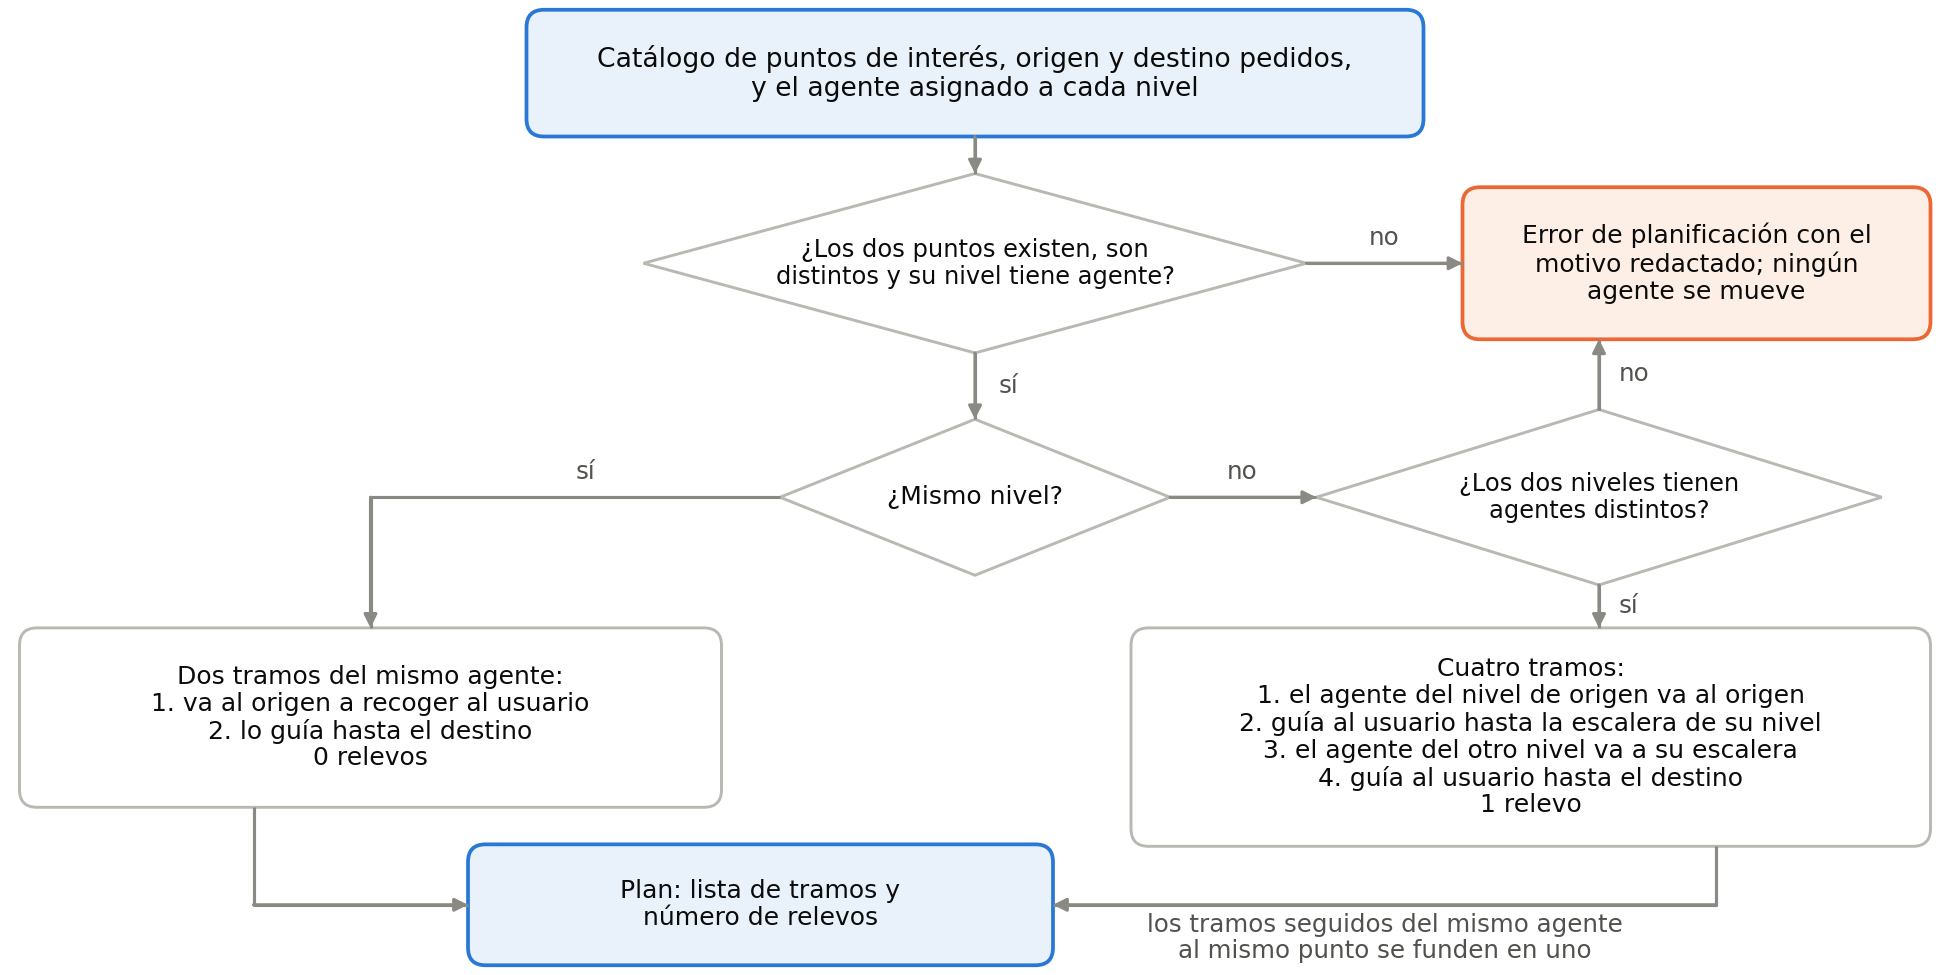
\includegraphics[width=0.84\textwidth]{imagenes/planificador.png}
  \caption{Función que planifica una misión. No usa ROS~2: recibe el catálogo, el origen, el destino y la asignación de un agente por nivel, y devuelve la lista de tramos o un error con su motivo, antes de que ningún agente se mueva.}
  \label{fig:planificador}
\end{figure}

Fue una de las decisiones más rentables del proyecto. Con el
relevo dentro del nodo, mezclado con los clientes de acción, la única forma de
comprobarlo habría sido levantar dos simuladores y observar si el agente llega.
Como función pura, una prueba automática la recorre entera en milisegundos y sin simulador. El catálogo de la simulación tiene 31 puntos de interés, y cada par ordenado de dos puntos distintos es una solicitud posible: $31 \times 30 = 930$ combinaciones de origen y destino. La prueba planifica las 930 y comprueba en todas que el plan empieza en el origen y termina en el destino, y que ningún agente recibe una meta fuera de su nivel. Comprueba también que una misión de un solo nivel usa un agente y ningún relevo, y que una de dos niveles usa los dos agentes y un relevo. Esa prueba encontró un defecto que
una corrida no habría delatado: cuando el origen o el destino era el propio punto
de transferencia de su nivel, el plan mandaba al mismo agente dos veces a la misma
pose. Nav2 devuelve éxito al instante ante un desplazamiento de cero metros, así
que en simulación no se habría visto.

\subsection{La asignación de tareas}
\label{sec:asignacion}

Cada nivel tiene un agente asignado, y esa correspondencia es un dato de
configuración, no una constante del código. El coordinador elige el agente al
aceptar la solicitud, según el nivel del origen y del destino. Con un solo agente
admisible por nivel no hace falta un optimizador, porque el método húngaro devolvería la misma tabla.

El planificador exige un único punto de transferencia por nivel y falla con un
mensaje explícito si encuentra dos. Hoy cada planta tiene una escalera y eso se
cumple; la verificación está para que, el día que haya dos, la decisión se tome a
la vista. En los agentes físicos, además, el coordinador no da por buena la llegada que
informa Nav2, sino que la comprueba con la pose que publica el agente.

\subsection{Escenarios de operación en simulación}
\label{sec:simulacion}

Los escenarios de varios pisos se construyeron primero en Gazebo~11 con ROS~2
Humble. La integración de Gazebo con ROS~2 en Humble aplica a todos los
complementos el espacio de nombres del primer modelo cargado. Por eso no fue posible tener dos agentes en un mismo proceso, y cada uno tiene su propio
simulador. El catálogo llegó a 31 puntos de interés: quince en el piso 2 y dieciséis en el piso 3 del edificio Gregorio.

Al principio los dos pisos estaban en un mismo mundo, y el láser simulado, de
10~m de alcance, veía paredes del otro piso en 61 de 1701 posiciones muestreadas. Esas posiciones estaban justo donde arranca el primer agente y donde está su punto de transferencia. Por
eso cada piso es ahora un mundo distinto, con su propio proceso de simulación. Los
dos agentes comparten un dominio de comunicaciones, separados por espacio de nombres, y la figura~\ref{fig:sim-relevo}
muestra una misión con relevo entre los dos procesos.

\begin{figure}[htbp]
  \centering
  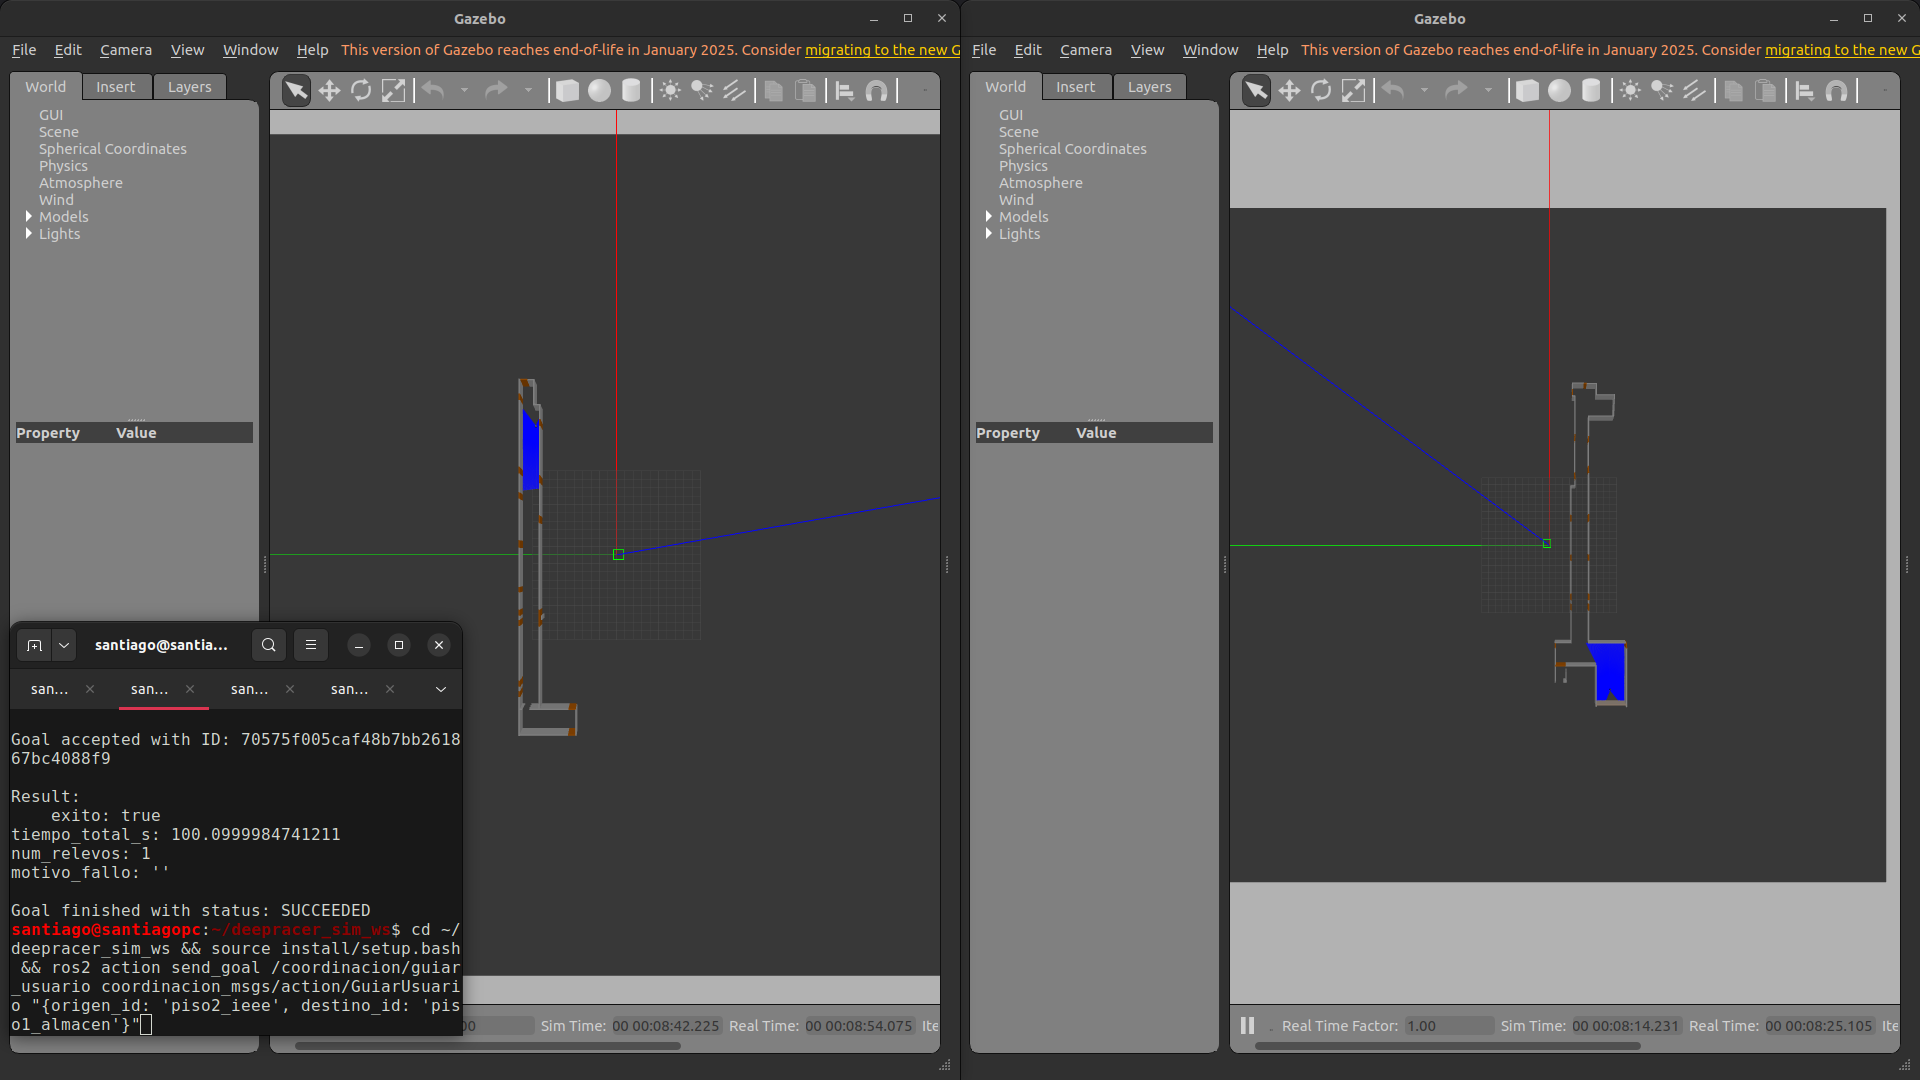
\includegraphics[width=\textwidth]{imagenes/simulacion_relevo_dos_procesos.png}
  \caption{Misión con relevo en simulación. Cada ventana es un proceso de Gazebo
    con un piso y su agente; el láser de cada uno se ve en azul. La terminal
    muestra el resultado de la acción: éxito, un relevo y 100,1~s de duración.}
  \label{fig:sim-relevo}
\end{figure}

El mapa de navegación tampoco salió de SLAM. El que se había construido cubría el
35,5~\% del largo del pasillo, medía 15,0~m de ancho frente a 5,3~m reales, y 2688
de sus 3618 celdas ocupadas, el 74~\%, no tenían ninguna pared detrás. Se reemplazó por un mapa calculado de la geometría del modelo, exacto en
simulación; como un mapa de ocupación es un corte horizontal, el del piso
superior resultó idéntico. Por último, la simulación debe correr a tiempo real
para que las métricas temporales valgan, y en las treinta misiones de la campaña
el factor de tiempo real tuvo un mínimo de 0,9917 y una media de 0,9973.

\subsection{De la simulación a los agentes físicos}
\label{sec:sim-a-vehiculos}

Al llevar el sistema a los agentes físicos se mantuvo su estructura: un coordinador, un
agente por piso, el relevo en la escalera y las reglas del contrato. También se mantuvo el código. El del coordinador,
el del planificador, el de los mensajes y el de la página es el mismo en los dos
destinos: compila sin cambios en las dos distribuciones de ROS~2 y completó una
misión en cada uno. Lo que cambió fue la implementación de los bloques. La
tabla~\ref{tab:sim-vehiculos} reúne cada cambio con su causa, y la
figura~\ref{fig:arquitectura-vehiculos} muestra el sistema como funcionó en la campaña con los agentes físicos.

\begin{table}[htbp]
  \centering\footnotesize
  \caption{Cambios en la implementación al pasar de la simulación a los agentes físicos.}
  \label{tab:sim-vehiculos}
  \begin{tabular}{@{}p{0.13\textwidth}p{0.21\textwidth}p{0.27\textwidth}p{0.31\textwidth}@{}}
    \toprule
    \textbf{Parte} & \textbf{En simulación} & \textbf{En los agentes físicos} & \textbf{Causa} \\ \midrule
    Distribución de ROS~2 & Humble en todos los componentes & Jazzy en los agentes y en el coordinador, que corre en un contenedor del portátil; Humble en la página y en rosbridge & El software de la tarjeta original solo existe para Ubuntu 24.04 con Jazzy, la simulación no existe en Jazzy, y la acción de navegación de Jazzy no es compatible con la de Humble \\ \addlinespace
    Coordinador & En el portátil, junto a los dos simuladores & En el portátil, después de un intento en uno de los agentes & Con el coordinador y el grabador en una tarjeta y las dos navegaciones encendidas, la carga subió de 6 a entre 17 y 33 y Nav2 no arrancaba \\ \addlinespace
    Comunicación & Un solo computador y un dominio de comunicaciones; un espacio de nombres por agente & Red inalámbrica con un punto de acceso de 5~GHz por piso; una partición por agente y topología en estrella hacia el portátil & Los tópicos del fabricante no llevan espacio de nombres, y los procesos de las dos cadenas, anunciándose por la red, saturaban las tarjetas \\ \addlinespace
    Locomoción & Complemento Ackermann de Gazebo con \texttt{ros2\_control} & Puente de la orden de velocidad a los servos, con una escala por agente & La tracción real tiene banda muerta y funciona en lazo abierto \\ \addlinespace
    Sensado & Láser simulado de 10~m de alcance & RPLIDAR A1M8 y la unidad inercial de la tarjeta; cámaras apagadas & Las cámaras no se usan y cargaban la tarjeta \\ \addlinespace
    Odometría & La del simulador & La del láser, combinada con la unidad inercial mediante un filtro & El agente no tiene codificadores en las ruedas, y con el láser solo el rumbo derivaba 5,9$^\circ$ por minuto \\ \addlinespace
    Mapa & Calculado de la geometría del mundo simulado & Derivado de la planta medida con flexómetro & El mapeo con SLAM a bordo no dio un mapa utilizable en ningún pasillo \\ \addlinespace
    Escenario & Pisos 2 y 3 del edificio Gregorio & Pisos 3 y 4 del edificio Calatayud, levantados con flexómetro & En Gregorio el tránsito de personas dificultaba las pruebas, el modelo no correspondía a la planta real y en sus pasillos uniformes la odometría del láser no veía el avance \\ \addlinespace
    Llegada & Tolerancia de 0,25~m & Tolerancia de 0,5~m, verificada con la pose del agente 1,5~s después de que Nav2 da la meta por alcanzada & Por la banda muerta, el agente no alcanza la precisión de la simulación, y sigue rodando cuando Nav2 declara la llegada \\ \addlinespace
    Media vuelta & La planifica Nav2, con marcha atrás & Maniobra propia del agente, vigilada con el láser y el mapa & En la salida del piso 4, de 2,5~m de ancho, la media vuelta de Nav2 abortó contra la pared \\ \bottomrule
  \end{tabular}
\end{table}

\begin{figure}[htbp]
  \centering
  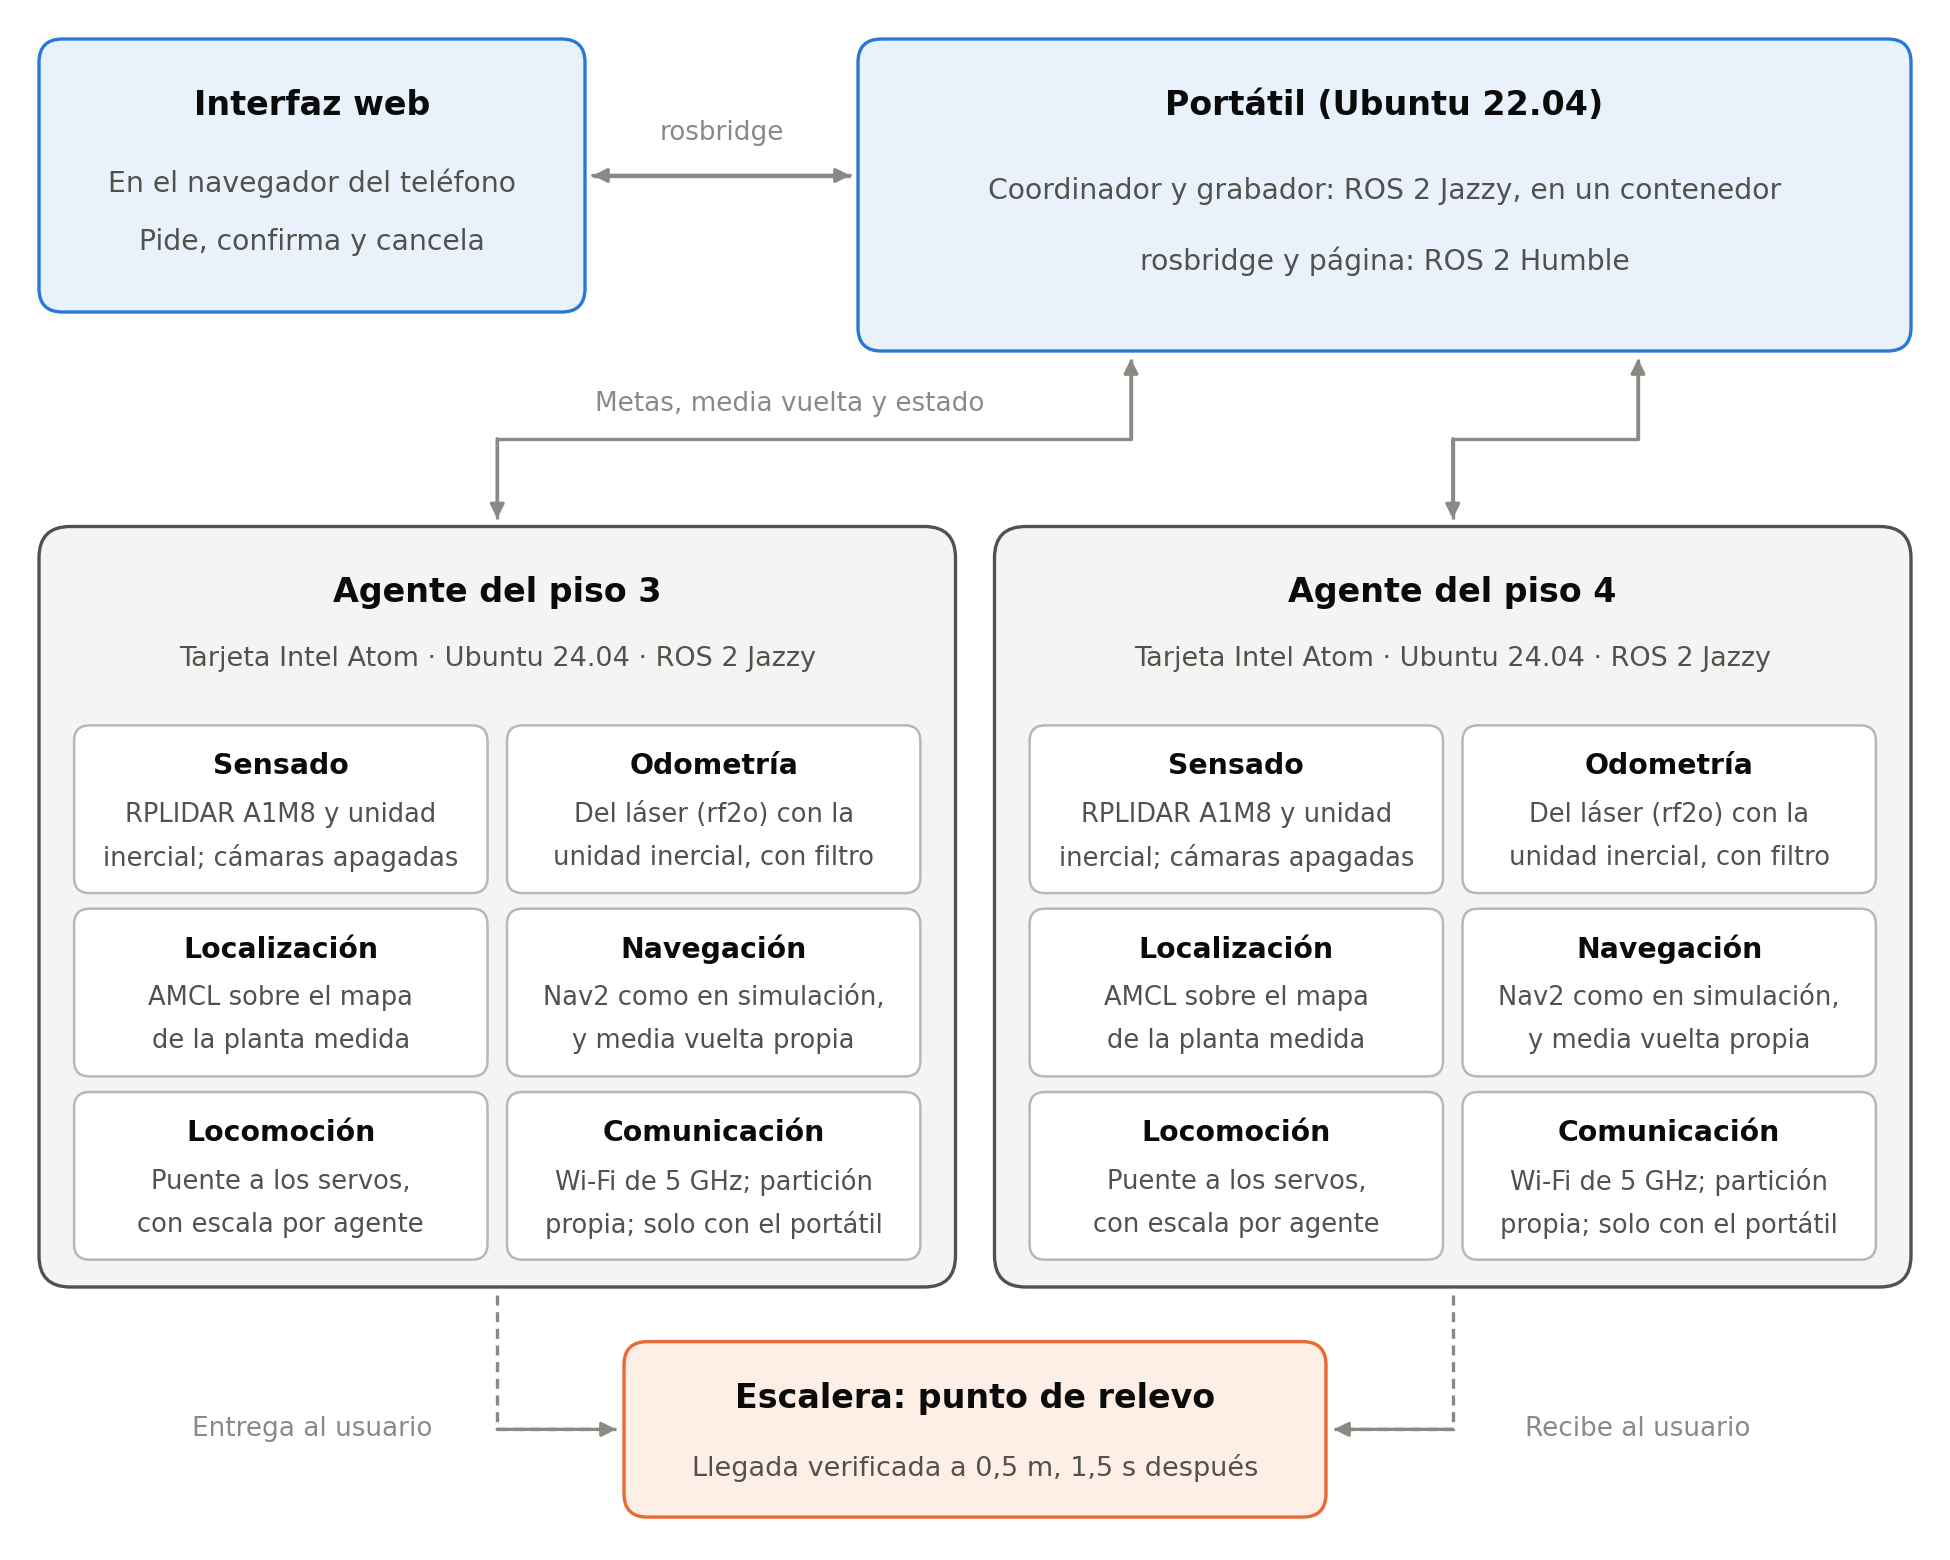
\includegraphics[width=0.86\textwidth]{imagenes/arquitectura_vehiculos.png}
  \caption{Arquitectura del sistema en la campaña con los agentes físicos, en los
    pisos 3 y 4. La estructura es la de la figura~\ref{fig:arquitectura}; cambia
    la implementación de los bloques.}
  \label{fig:arquitectura-vehiculos}
\end{figure}

% =====================================================================
\section{Plataforma robótica}
\label{sec:plataforma}

\subsection{Componentes del agente}
\label{sec:componentes}

Los dos agentes operan con su tarjeta original, para la que el software de la
comunidad solo se publica sobre Ubuntu 24.04 con ROS~2 Jazzy. La
tabla~\ref{tab:vehiculo} reúne los componentes. Cada agente atiende un piso del edificio Calatayud, uno el 3 y otro el 4. El láser que traía el kit no era el que describía el primer
informe de hardware; se identificó leyendo el modelo que reporta el propio
sensor.

\begin{table}[htbp]
  \centering\small
  \caption{Componentes de cada agente y del computador central.}
  \label{tab:vehiculo}
  \begin{tabular}{@{}p{0.25\textwidth}p{0.68\textwidth}@{}}
    \toprule
    \textbf{Componente} & \textbf{Descripción} \\ \midrule
    Chasis & AWS DeepRacer, escala 1:18, dirección Ackermann, motor de tracción con variador y servomotor de dirección \\ \addlinespace
    Cómputo & Tarjeta original, procesador Intel Atom E3930 de dos núcleos, 4~GB de memoria; Ubuntu 24.04 y ROS~2 Jazzy \\ \addlinespace
    Láser & RPLIDAR A1M8-R5: 360$^\circ$, 360 muestras por barrido, alcance de 0,15 a 12~m, entre 6,8 y 7~Hz \\ \addlinespace
    Unidad inercial & Bosch BMI160 integrada en la tarjeta, por I2C: giroscopio y acelerómetro \\ \addlinespace
    Cámaras & Estéreo; desactivadas por software, porque el sistema no las usa y cargaban la tarjeta \\ \addlinespace
    Alimentación & Una batería para el cómputo y otra de polímero de litio para la tracción \\ \addlinespace
    Computador central & Portátil con Ubuntu 22.04 y ROS~2 Humble (AMD Ryzen 5 PRO 5650U, 16~GB); el coordinador corre en un contenedor con Jazzy \\ \bottomrule
  \end{tabular}
\end{table}

\subsection{Nav2 sobre un agente que no gira sobre su eje}
\label{sec:nav2-ackermann}

La configuración por omisión de Nav2 asume tracción diferencial y propone
trayectorias que un vehículo tipo automóvil no puede ejecutar. Por eso se sustituyeron dos de sus tres capas. La
planificación global pasó al planificador híbrido A* de Smac con modelo
Reeds-Shepp, y el seguimiento, al controlador Regulated Pure Pursuit, los
dos con marcha atrás, y con una velocidad deseada de 0,5~m/s. Del árbol de
comportamiento se quitó la recuperación que gira sobre el propio eje, con la que
el agente, ante un bloqueo, movía las ruedas sin avanzar hasta agotar los
reintentos. Los parámetros tienen una variante por distribución, y una prueba
automática falla si se separan en algo distinto de las diferencias documentadas.

La cadena se puso en marcha con la escalera de siete pasos de la guía oficial de
Nav2 \autocite{nav2setup}. El orden va de las transformaciones entre marcos de referencia al
planificador y el controlador, pasando por la odometría, el láser, el mapa, la
localización y los mapas de costos. Seguir ese orden permitió aislar el problema de la odometría, porque una odometría que no mide y un planificador que no
planifica se manifiestan igual: el agente no llega. El orden importa también al
arrancar, porque los mapas de costos leen el mapa al configurarse. Por eso el
programa de arranque de los agentes activa primero el servidor de mapas y
espera a que los seis nodos de la cadena estén activos. En el laboratorio, la
cadena quedó lista en 4~min 4~s en un agente y en 4~min 22~s en el otro.

\subsection{La odometría del láser como limitación principal}
\label{sec:odometria-laser}

El agente no tiene codificadores en las ruedas, y su única odometría sale de
comparar barridos sucesivos del láser. Desde que se midió por primera vez, el 26 de agosto en simulación, hasta el cambio de edificio, el 2 de octubre, no dio una medida utilizable, por falta de información en la señal: en un pasillo recto y uniforme, cada barrido es casi idéntico al anterior y el estimador devuelve un avance cercano a cero. En los pasillos del edificio Gregorio la odometría registró desde el 1,3~\% del avance real, en simulación, hasta el 73~\%, con un agente físico en el hall del piso 3, y la localización llegaba a separarse más de dos metros de la
posición medida con flexómetro (figura~\ref{fig:hall}).

\begin{figure}[htbp]
  \centering
  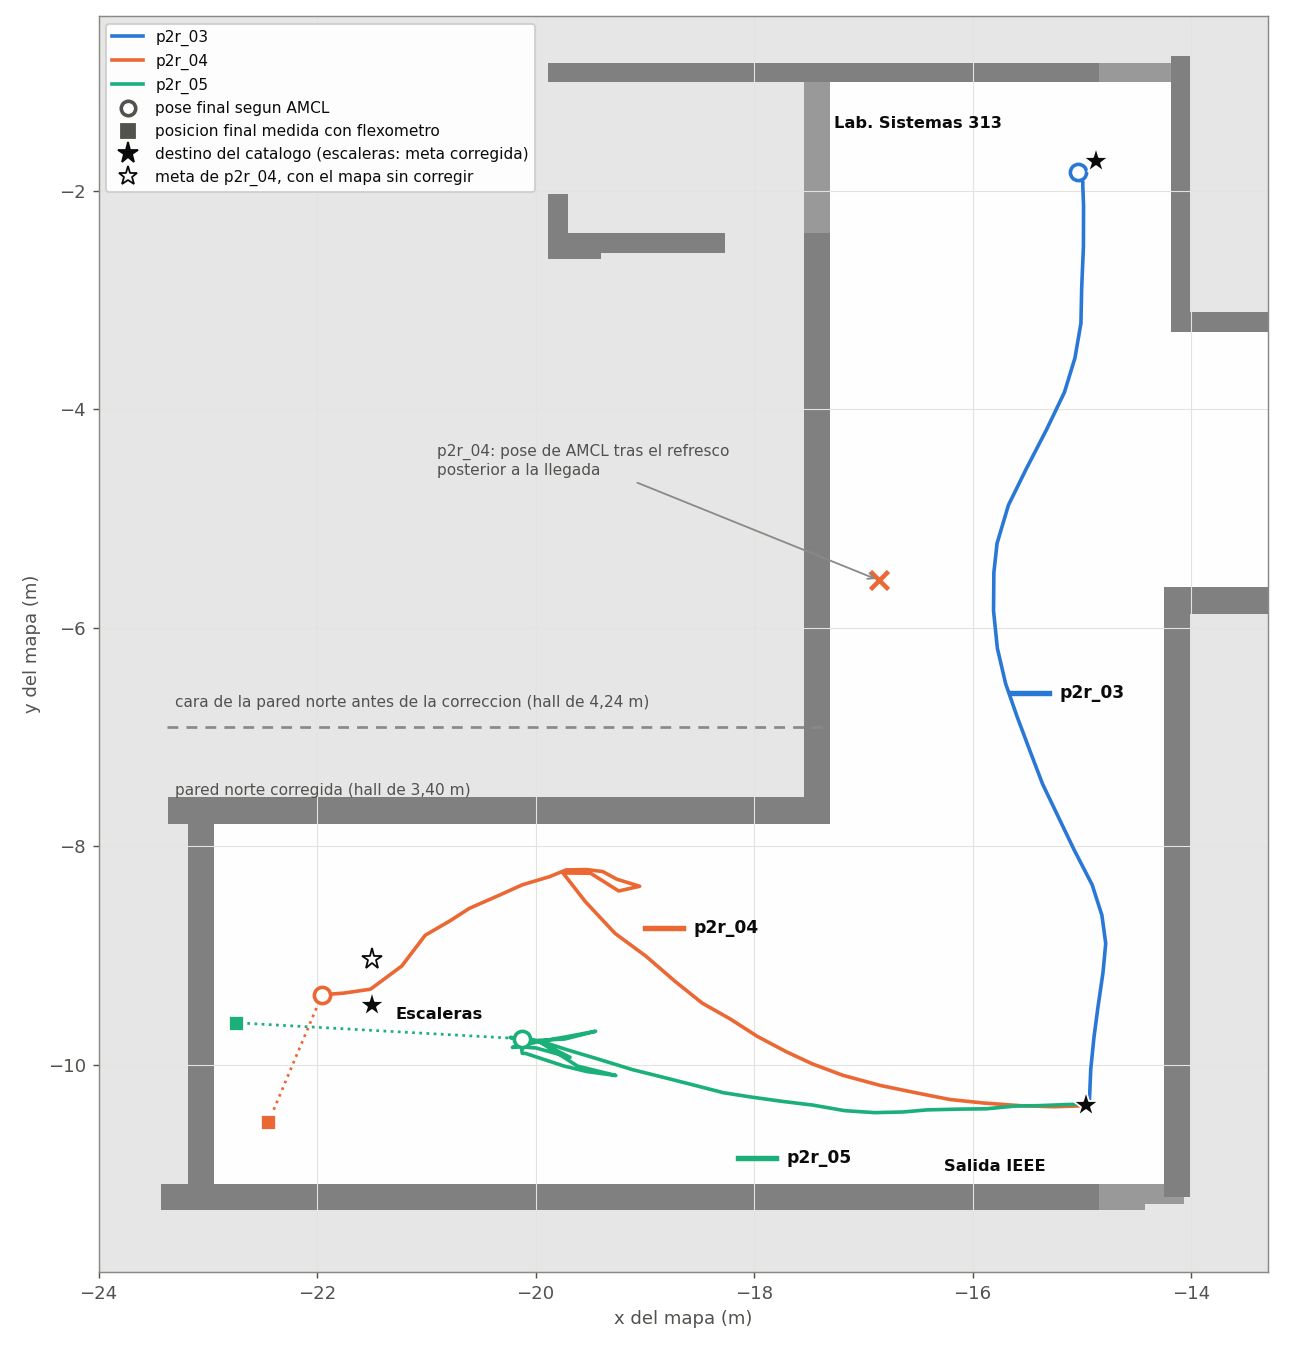
\includegraphics[width=0.6\textwidth]{imagenes/recorridos_hall_piso2.png}
  \caption{Tres recorridos de un agente en el hall del piso 3 del edificio Gregorio. El círculo es la pose que
    reporta la localización al terminar; el cuadrado, la posición real medida con
    flexómetro. La separación entre los dos es el error, y su causa está en la
    odometría, no en el algoritmo de localización.}
  \label{fig:hall}
\end{figure}

Ningún ajuste del algoritmo recupera información que la señal no contiene, y por
eso la solución fue cambiar de entorno. El criterio salió de la misma medida:
hace falta estructura no uniforme dentro del alcance del sensor durante todo el
recorrido. Los pisos 3 y 4 del edificio Calatayud la tienen. Entre las hornacinas de los salones, los
casilleros, la papelera, el ascensor y la escalera suman ocho cambios de perfil en
25~m, uno cada tres metros. Con la misma odometría y sin cambiar un parámetro, el error cayó por debajo del 5~\% (tabla~\ref{tab:odometria}). El cambio de edificio fue la decisión que hizo posible la demostración física, porque en los pasillos de Gregorio ningún ajuste habría dado al agente la información que le faltaba.

\subsection{Los mapas, derivados de medidas y no de SLAM}
\label{sec:mapas}

Los intentos de construir el mapa con SLAM en los propios agentes, en septiembre, no dieron un mapa utilizable en ningún pasillo, por la misma falta de información de avance. La vía que
funcionó fue levantar la planta con flexómetro y derivar de ese levantamiento
tanto el mundo simulado como el mapa de navegación. Así, simulación y edificio
coinciden porque salen de la misma fuente. Esa correspondencia se había dado por
supuesta, y al verificarla por primera vez resultó falsa. El modelo del edificio Gregorio daba el hall del piso 3 0,84~m más ancho de lo que es, 4,24~m frente a 3,40~m, un 25~\% de error. En los pisos 3 y 4 de Calatayud se invirtió el orden: primero se midió y después se modeló.

La herramienta que genera las plantas suma las dos paredes de cada pasillo y
avisa si no cierran dentro del 2~\%. Esa comprobación encontró cinco errores antes
de generar nada, y las dos plantas cierran al 0,32~\% y al 0,62~\%. La
figura~\ref{fig:mapa4} es el mapa del piso 4, con sus cinco puntos de interés:
tres salones, el ascensor y la escalera, que es su punto de transferencia.

\begin{figure}[htbp]
  \centering
  \includegraphics[width=\textwidth]{imagenes/mapa_piso4.png}
  \caption{Mapa de navegación del piso 4, derivado del levantamiento con
    flexómetro. El pasillo corre 25~m del extremo norte al sur; los salones
    quedan al este, y el ascensor y la escalera al oeste.}
  \label{fig:mapa4}
\end{figure}

\subsection{La banda muerta de tracción}
\label{sec:banda-muerta}

Al integrar la cadena de tracción apareció una característica de la plataforma
que condiciona la llegada: el agente no se mueve con velocidades pedidas por
debajo de 0,40~m/s. El puente que traduce la orden al variador las convertía en
tracción nula, sin ningún aviso, y el agente se detenía al entrar en la fase
final del recorrido, intentando moverse a una velocidad que su propia cadena
anulaba. Se subió a 0,40~m/s la velocidad mínima de aproximación del controlador,
y después se modificó el puente para que envíe las órdenes menores con el escalón
de tracción más bajo.

El resultado es que el agente se aproxima a la meta a 0,40~m/s y no tiene
régimen de aproximación fina. Es un límite de la plataforma, que no se corrige
afinando el controlador. Como la tracción funciona en lazo abierto, la relación
entre la orden y la velocidad real tampoco es igual en los dos agentes. Por eso el puente tiene una escala por agente, ajustada en campo: 0,85 en el del piso 3 y
0,9 en el del piso 4. Con la escala 1,0, el del piso 4 iba a 1,36~m/s y se pasaba
de la meta; con 0,9 va a 0,74~m/s.

Ante ese límite, la tolerancia de llegada con los agentes físicos se fijó en 0,5~m antes de las pruebas de navegación, mientras la simulación conserva 0,25~m.

\subsection{La unidad de medición inercial de la tarjeta}
\label{sec:imu}

Al principio el rumbo también salía de la odometría del láser, que en un pasillo
recto pierde los giros igual que el avance. Con el agente quieto, ese rumbo
derivó hasta 5,9$^\circ$ por minuto, y un giro de 90$^\circ$ hecho a mano se
registró como 19,1$^\circ$. La tarjeta incluye una unidad de medición inercial,
una Bosch BMI160 que el software del fabricante no usa. Leída directamente, midió
giros de 90$^\circ$ y 360$^\circ$ con un error de 0,1~\% a 1,3~\%, y quieta no se
desvió más de 0,3$^\circ$ en 60~s.

Se escribió un nodo que la lee y calibra el sesgo del giroscopio al arrancar. Un filtro de Kalman extendido toma de la
odometría del láser el avance y de la unidad inercial el giro; la unidad publica
a 25~Hz y el filtro corre a 15~Hz, para no cargar la tarjeta. En un giro de
90$^\circ$ contra una línea del piso, el filtro midió 90,17$^\circ$ en un agente
y 88,38$^\circ$ en el otro, y con el agente quieto su rumbo se movió
0,3$^\circ$ o menos por minuto. La posición no mejora, porque sigue saliendo del
láser. Con el rumbo estable se redujo de 1,0 a 0,5~m el margen en el que Nav2 da
la meta por alcanzada, y con ese margen se superó la prueba de navegación de un agente.

\subsection{Los dos agentes en la misma red}
\label{sec:dos-vehiculos}

Con los dos agentes encendidos aparecieron tres problemas que con uno solo no
existían. El primero fue de permisos. El software del fabricante se ejecuta con
el usuario administrador, y ROS~2 intercambia los datos entre procesos del mismo
equipo por memoria compartida, a la que solo ese usuario puede escribir. Los
programas lanzados con otro usuario veían los nodos del fabricante pero no podían
intercambiar mensajes con ellos, sin ningún error, y durante tres semanas eso
pareció una avería de uno de los agentes.

El segundo fue de nombres. Los tópicos del fabricante no llevan espacio de
nombres, así que una orden de movimiento llegaba a los dos agentes y la
odometría de cada uno recibía el láser del otro. Cada agente tiene ahora una
partición de comunicaciones propia, y la cadena del proyecto corre con un espacio
de nombres distinto en cada uno.

El tercero apareció en el primer intento de misión con relevo. Con las dos cadenas completas, todos sus procesos se anunciaban unos a otros por la red inalámbrica. La carga de la tarjeta de un agente pasó de 6 a entre 17 y 33, con
el procesador al 84--95~\%, y Nav2 no llegaba a arrancar. La respuesta fue la topología en estrella del diseño: los procesos de
cada agente solo se buscan dentro de él, lo que el coordinador necesita solo se
anuncia al portátil, y los agentes no se ven entre sí. El coordinador y el
grabador pasaron al portátil, en un contenedor con Jazzy, y verifican las
llegadas con la pose que cada agente publica dos veces por segundo.

Con todo el sistema en el laboratorio, las tarjetas quedaron al 54~\% y al 59~\%
de uso en reposo, y al 68~\% y al 74~\% navegando con las ruedas en el aire. El controlador de Nav2, que corre a 10~Hz, no bajó de 5,5~Hz. La red tiene un punto
de acceso de 5~GHz por piso, en la misma subred. Entre los dos agentes, el
tiempo de ida y vuelta de los mensajes tuvo una mediana de 5,99~ms y un percentil
95 de 11,12~ms, sin pérdidas, frente al límite de 100~ms que fija el requisito.

\subsection{La media vuelta en varios tiempos}
\label{sec:media-vuelta}

Como en la operación real, cada misión empieza donde terminó la anterior, y
el siguiente usuario queda a menudo detrás del agente, que en pasillos de 2,5 a
3,2~m de ancho tiene que dar la vuelta en varios tiempos. En el piso 4, a la
salida del pasillo de 2,5~m, la media vuelta de Nav2 abortó dos veces contra la
pared, porque el planificador proponía cada segundo una maniobra distinta.
Además, con la misma orden, el motor retrocedía a 1,7 veces la velocidad de avance, y se añadió
al puente una escala de 0,75 para la marcha atrás.

La media vuelta se escribió como una maniobra propia del agente, en lugar de seguir ajustando Nav2, que en ese caso trabajaba en el borde de lo que su controlador resuelve. La maniobra alterna
marcha atrás y avance con la dirección a tope y empieza hacia el costado con más
espacio. Cada tiempo se corta cuando la huella prevista del agente queda a
menos de 0,10~m de un obstáculo, visto por el láser o marcado en el mapa, donde la
escalera está cerrada porque el láser no ve su borde.

El coordinador la pide antes de una meta que queda a más de 110$^\circ$ del rumbo
del agente y a más de 1,5~m, y si no se completa en 120~s, sigue Nav2. En sus
primeras pruebas giró 160$^\circ$ y 167$^\circ$, en un solo tiempo cada vez, y en la campaña con los agentes físicos se ejecutó 24 veces.

% =====================================================================
\section{Interfaz de interacción con el usuario}
\label{sec:oe3}

\subsection{Una página web, no una aplicación}

El objetivo pide «una interfaz móvil», y se construyó una página web que se abre en el navegador del teléfono. Para el usuario que el proyecto declara, cumple el objetivo mejor que una aplicación, porque un visitante ocasional
no va a instalar nada para preguntar por un salón. La página funciona sin salida
a internet, porque la red del edificio puede no tenerla, y no usa bibliotecas ni
recursos externos. Son un archivo HTML, una hoja de estilo y dos programas en JavaScript, que sirve el propio portátil. Se comunica con
ROS~2 por el puente \textit{rosbridge}, que no tiene autenticación, así que el firewall del portátil solo admite conexiones desde la red de los agentes.

El primer programa es un cliente propio del protocolo del puente, porque la
biblioteca de cliente más difundida implementa las acciones de la primera generación de ROS. El segundo es la lógica de la página. Recibe el catálogo de puntos al conectarse y el estado de la misión una
vez por segundo, pide y cancela con la acción de guiado y publica la
confirmación de cambio de piso.

\subsection{Lo que el usuario ve}

El usuario elige el origen en una lista y el destino en un catálogo con búsqueda
por nombre, donde cada destino muestra su piso y, si queda en el otro nivel, la
marca «con relevo». Durante la misión, la página muestra un título calculado a
partir de la etapa, el texto que redacta el coordinador, el agente que está
guiando, hacia dónde va, el destino final y la distancia restante. Una franja de
cinco pasos (preparando, tramo 1, relevo, tramo 2 y fin) marca el paso actual (figura~\ref{fig:hri}, izquierda).

\begin{figure}[!htbp]
  \centering
  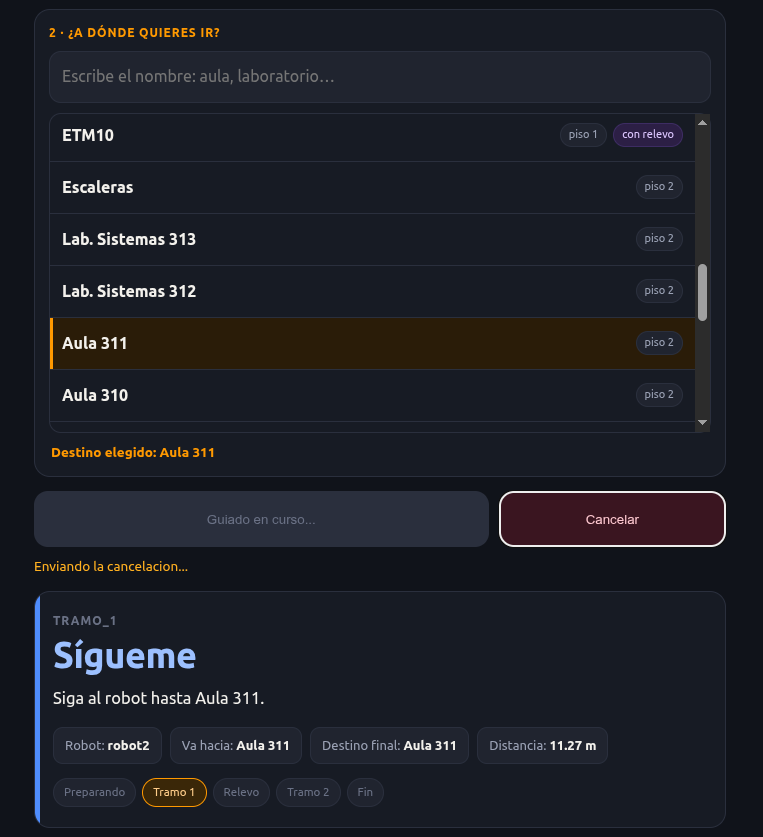
\includegraphics[height=8.4cm]{imagenes/hri_seguimiento.png}\hspace{0.04\textwidth}%
  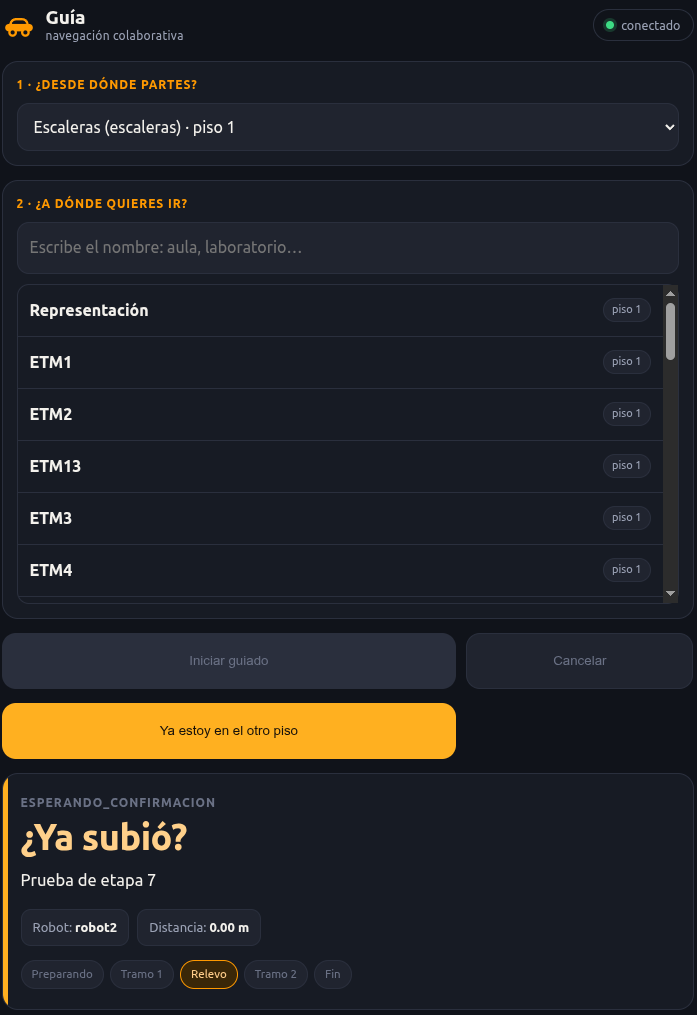
\includegraphics[height=8.4cm]{imagenes/hri_confirmacion_piso.png}
  \caption{Interfaz web. A la izquierda, durante una misión en simulación: el destino elegido, el botón de cancelar y el panel de estado del primer tramo, con el texto del coordinador, el agente activo y la distancia restante. A la derecha, en la etapa de espera de confirmación, durante su prueba automática: el estado lo publica la prueba, con el texto «Prueba de etapa 7», y la página muestra el botón «Ya estoy en el otro piso», de la versión anterior a los ajustes que siguieron a las pruebas con los agentes físicos.}
  \label{fig:hri}
\end{figure}

La interfaz se verificó contra el coordinador real: el catálogo, una misión con
sus etapas, el texto del coordinador mostrado literal y el botón que se reactiva
al terminar. También se operó una misión completa con relevo desde un teléfono
real conectado a la red de los agentes, sin tocar el computador. Las dos
funciones que siguen se añadieron después de ver el sistema en uso.

\subsection{Confirmación de cambio de piso}

En una misión entre niveles, el segundo agente llega a su escalera y espera al
usuario, pero no puede saber si la persona ya subió. Sin una pausa explícita, la
misión podía darse por completada con el usuario todavía en el piso equivocado, y
la instrumentación lo habría registrado como éxito. Por eso, cuando el segundo
agente llega a su punto de transferencia, el coordinador pasa a la etapa de espera de confirmación. La página muestra entonces un botón para confirmar el cambio de
piso, que solo existe en esa etapa (figura~\ref{fig:hri}, derecha). A los 60~s sin
confirmación aparece un aviso, y a los 120~s la misión termina como fallida. Los
plazos se cuentan desde que llega el agente, para que un agente lento no le
consuma tiempo al usuario, y se miden con el reloj del sistema y no con el de la
simulación. Si el usuario confirma antes de que el agente llegue, la
confirmación se retiene y se aplica al llegar.



Se verificó en simulación con una corrida por camino. Confirmar a los pocos segundos termina la misión con éxito, y confirmar pasados los 60~s hace aparecer el aviso en el teléfono. No confirmar deja la misión fallida a los 120~s, con el
motivo redactado.

\subsection{Cancelación}

El botón de cancelar existía pero no hacía nada, y no se había detectado. El
servidor de acción del coordinador no registraba la función que responde a la
cancelación, y ROS~2 rechaza por omisión, sin informar, toda cancelación que no
tenga esa función. Al corregirlo se añadió el comportamiento que faltaba: la
misión pasa por la etapa de cancelación, el agente activo regresa al punto de
transferencia de su piso, y la misión cierra como fallida con un texto que lo
dice. En simulación, con una corrida cancelada y una de control, el agente
quedó a 0,121~m de su punto de regreso.

Con los agentes físicos se cancelaron seis misiones, al menos una en cada etapa, y en
las seis el agente volvió a su escalera, a entre 0,07 y 0,34~m de su punto. Esas
pruebas mostraron un defecto que la simulación no podía mostrar, porque la media
vuelta propia se añadió después. Nav2 conserva durante un tiempo las metas terminadas, y mientras tenía una cancelada en su lista, el agente se declaraba en error y rechazaba la media vuelta. Sin ella, Nav2 intentaba girar
por su cuenta en el pasillo y oscilaba. Ahora la media vuelta solo espera a que no
haya una meta en curso: antes de la corrección se rechazaron ocho de quince
medias vueltas, y después ninguna de diez.

\subsection{Ajustes tras las pruebas con los agentes físicos}
\label{sec:ajustes-campo}

Las pruebas con los agentes físicos mostraron tres defectos de la página. El título de
la etapa de confirmación preguntaba siempre «¿Ya subió?», lo que al subir
resultaba brusco y al bajar del piso 4 al 3 era falso. Ahora sale de comparar el
piso de origen con el del agente que espera, como «Suba con calma al piso 4» o «Baje con calma al piso 3». El botón dice «Ya estoy en el piso 4», o el piso que
corresponda.

Ese cambio se hizo el día de la campaña, antes de correrla, y aun así los
teléfonos mostraron la versión anterior, porque el servidor no le indicaba al
navegador cuándo volver a pedir la página. Ahora la página se sirve con la
indicación de comprobarla cada vez que se abre. El tercer defecto fue de nombres:
los dos ascensores se llamaban igual en la lista y en una misión se eligió el del
piso equivocado, así que los nombres repetidos se muestran ahora con su piso, como
«Ascensor (piso 3)». Los tres ajustes se verificaron con pruebas automáticas y
después con un teléfono y los agentes físicos, en una misión de subida y otra de
bajada.

% =====================================================================
\section{Protocolo experimental e instrumentación}
\label{sec:protocolo}

El protocolo se escribió antes de instrumentar el sistema, a propósito: un protocolo redactado después
de ver los datos tiende a acomodarse a lo que salió, por ejemplo eligiendo el
umbral que deja fuera las corridas malas. El protocolo fija las métricas con su
definición operativa, el criterio de éxito, el tamaño de muestra y una lista
cerrada de causas de descarte, y cada versión queda fechada en el historial del
repositorio.

\subsection{Definiciones operativas}

Una métrica sin un evento de inicio y uno de fin medibles por una máquina no se
puede reportar. La tabla~\ref{tab:metricas} da los dos eventos de cada una. Todas
las marcas salen de un mismo reloj: en simulación, el de la simulación; en los agentes físicos, el del computador que graba.

\begin{table}[htbp]
  \centering\small
  \caption{Definición operativa de las cuatro métricas del anteproyecto.}
  \label{tab:metricas}
  \begin{tabular}{@{}p{0.2\textwidth}p{0.36\textwidth}p{0.36\textwidth}@{}}
    \toprule
    \textbf{Métrica} & \textbf{Inicio} & \textbf{Fin} \\ \midrule
    Tiempo de respuesta & El coordinador acepta la solicitud & Primera de tres muestras seguidas de la odometría del agente asignado con velocidad de al menos 0,02~m/s \\ \addlinespace
    Tiempo de asignación & Primera publicación de la etapa recibida & Primera publicación del primer tramo, con el agente asignado \\ \addlinespace
    Tasa de éxito & \multicolumn{2}{p{0.72\textwidth}}{Proporción de misiones exitosas sobre las corridas válidas} \\ \addlinespace
    Continuidad entre niveles & El primer agente alcanza su punto de transferencia & Primer movimiento del segundo agente \\ \bottomrule
  \end{tabular}
\end{table}

Una misión es exitosa si cumple tres condiciones. La pose final del agente, en
su odometría, está a 0,25~m o menos del destino declarado en el catálogo; en los agentes físicos el umbral es de 0,5~m. La misión llegó a la etapa completada sin pasar
por fallida. Y, si era entre niveles, hubo un relevo.

La regla central del protocolo es que el éxito se mide contra
la odometría del agente, nunca contra el resultado que devuelve Nav2. Una
navegación puede terminar en éxito y haber dejado al agente lejos del destino:
en las primeras pruebas en simulación, una de tres metas devolvió éxito con el
agente a 0,296~m. Aceptar ese resultado sería dejar que el sistema se evalúe a
sí mismo.

El tiempo de asignación resultó menor que el paso de 100~ms del reloj de la
simulación, así que se reporta como una cota por misión y se caracterizó aparte,
en un banco de pruebas con el reloj del sistema. La continuidad se definió primero como una condición binaria, que resultó no poder fallar, y se reemplazó por el intervalo del relevo, una magnitud que sí varía.

\subsection{Diseño de la campaña en simulación}

La campaña en simulación tiene treinta misiones en dos grupos de quince. En las de un mismo piso, el origen y el destino están en el mismo nivel y no hay relevo; sirven de comparación. En las de dos pisos hay un relevo, y son las que responden la pregunta de investigación.

Los pares de origen y destino salen de un sorteo, porque con pares elegidos a mano se corre el riesgo de probar justo los recorridos que funcionan. Se sortean entre los puntos del catálogo menos los dos puntos de transferencia, catorce en el piso 2 y quince en el piso 3, que dan 392 pares posibles dentro de un mismo piso y 420 entre pisos, y ningún par se repite. La semilla del sorteo es la fecha en que se hace, escrita como año, mes y día, y el listado se guarda en el repositorio antes de la primera corrida. Así, nadie puede probar semillas hasta obtener un sorteo conveniente.

Las diez primeras misiones salieron de un sorteo con la semilla 20260822 en el que todas las misiones entre pisos subían del piso 2 al 3 y todas las de un solo piso se quedaban en el 2. El grupo con relevo era el único que navegaba por el piso 3, y una diferencia entre los grupos no habría podido atribuirse al relevo. Las veinte restantes se sortearon de nuevo el 4 de septiembre, con la semilla 20260904, para que cada grupo quedara repartido entre los dos pisos: en el de un mismo piso, ocho misiones en el piso 2 y siete en el 3; en el de dos pisos, ocho de subida y siete de bajada.

Una corrida fallida cuenta como fallo. Solo se descarta si la causa es ajena al sistema y está en una lista cerrada, escrita antes de la campaña, que admite la caída del simulador, un controlador del agente que no
se activa, el factor de tiempo real por debajo de 0,99, un fallo de la máquina
anfitriona o una cancelación por una causa externa anotada antes de conocer el
resultado. Si los descartes superan el 20~\% de las corridas, la campaña no es
válida.

\subsection{Instrumentación}
\label{sec:instrumentacion}

Cada misión deja una grabación de datos de ROS (\textit{rosbag}) con los tópicos
del coordinador y de los dos agentes. Un programa compone a partir de ella el
registro de la misión, en un formato estructurado que se valida contra un esquema versionado. El registro contiene las marcas de cada etapa, la trayectoria de cada agente, la pose
final, el error de llegada y su procedencia. Un segundo programa comprueba la
integridad de los registros y calcula las cuatro métricas con sus intervalos de
confianza. Se escribió antes de la campaña, y encontró dos defectos que después
habrían sido irreparables: la continuidad no tenía campo en el esquema, y el
intervalo que citaba el protocolo no se reproducía con el método declarado.

Con los agentes físicos, el grabador corre en el contenedor con Jazzy, y un programa adapta la grabación al formato que leen las
herramientas de Humble. El registro usa el reloj del computador, la tolerancia de
0,5~m y el mapa de cada piso. La llegada la verifica el coordinador con la pose que publica el agente, 1,5~s después de que Nav2 la da por alcanzada (figura~\ref{fig:instrumentacion}). Nav2 la declara en cuanto el agente entra en su margen, y el agente sigue rodando.
En las llegadas medidas en el piso 4, el agente estaba a entre 0,53 y 0,62~m de
la meta en la última orden de avance, y un segundo después, ya quieto, a entre
0,09 y 0,53~m. La distancia de llegada se guarda con su procedencia, medida con
flexómetro o tomada de la localización del agente, y el analizador advierte cuando no hay medida externa, como ocurrió en la campaña con los agentes físicos.

\begin{figure}[!htbp]
  \centering
  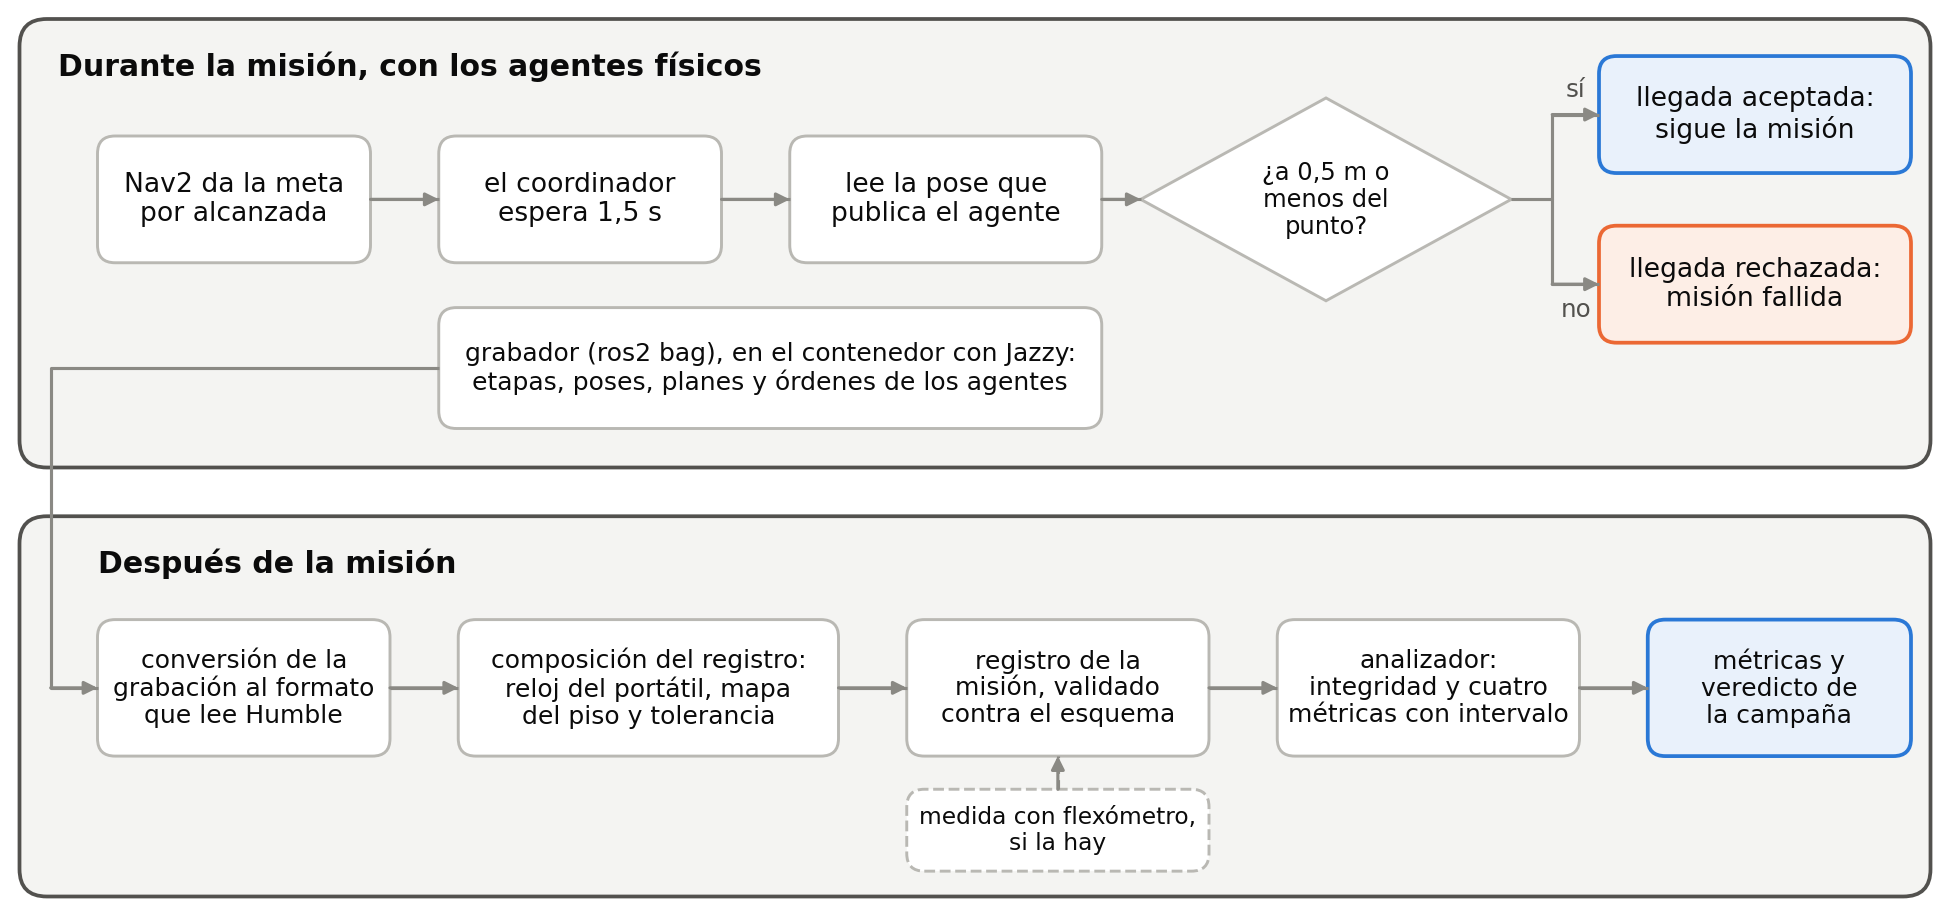
\includegraphics[width=\textwidth]{imagenes/instrumentacion.png}
  \caption{Instrumentación de una misión. Arriba, la verificación de la llegada que hace el coordinador con los agentes físicos; abajo, el camino de la grabación hasta las métricas de la campaña. En simulación el camino es el mismo, sin la conversión de formato y con la tolerancia de 0,25~m.}
  \label{fig:instrumentacion}
\end{figure}

\subsection{Pruebas de verificación de la demostración física}
\label{sec:pruebas-verificacion}

La demostración con los agentes físicos se organizó en seis pruebas de verificación
sucesivas. Cada prueba tiene un criterio escrito antes de correrla y lo que
significa no superarla (tabla~\ref{tab:pruebas-verificacion}). Se fijaron tres
fechas de revisión en octubre, y después de la última, el 16 de octubre, no se
toman más datos.

\begin{table}[htbp]
  \centering\small
  \caption{Pruebas de verificación de la demostración física y su estado al
    cerrar la toma de datos.}
  \label{tab:pruebas-verificacion}
  \begin{tabular}{@{}p{0.24\textwidth}p{0.52\textwidth}p{0.16\textwidth}@{}}
    \toprule
    \textbf{Prueba} & \textbf{Criterio} & \textbf{Estado} \\ \midrule
    Actuación & El agente responde a las órdenes de dirección y tracción & Superada \\ \addlinespace
    Odometría & Error de 10~\% o menos sobre un recorrido conocido de 5~m o más & Superada \\ \addlinespace
    Navegación de un agente & Un agente llega de un punto a otro con Nav2, con la llegada verificada & Superada \\ \addlinespace
    Dos agentes en la misma red & Los dos agentes y el coordinador coexisten sin conflicto de nombres & Superada \\ \addlinespace
    Misión con relevo & Una misión con relevo sobre los dos agentes, con su registro & Superada \\ \addlinespace
    Campaña con los agentes físicos & Entre 5 y 10 repeticiones del protocolo con su registro & Superada \\ \bottomrule
  \end{tabular}
\end{table}

Para la campaña con los agentes físicos se sortearon el 13 de octubre, con la semilla 20261013, diez misiones entre los pisos 3 y 4 del edificio Calatayud: cinco de subida y cinco de bajada. Se corrieron en ese orden y sin reubicar los agentes entre misiones, como ocurriría en la operación real.
